% !TEX program = xelatex
\documentclass[11pt,a4paper]{ctexart}

% ── 字体 ──
\setCJKmainfont{STSong}
\setCJKsansfont{PingFang SC}
\setCJKmonofont{STFangsong}

% ── 宏包 ──
\usepackage[margin=2.5cm]{geometry}
\usepackage{amsmath,amssymb,amsthm}
\usepackage{graphicx}
\usepackage{booktabs}
\usepackage{hyperref}
\usepackage{xcolor}
\usepackage{enumitem}
\usepackage{float}
\usepackage{caption}
\usepackage{subcaption}
\usepackage{url}
\usepackage[numbers,sort&compress]{natbib}
\hypersetup{
  colorlinks=true,
  linkcolor=blue!70!black,
  citecolor=green!50!black,
  urlcolor=blue!60!black,
}

% ── 图表路径 ──
\graphicspath{{../results/figures/}}

% ── 定理环境 ──
\newtheorem{proposition}{命题}

% ── 标题 ──
\title{\textbf{OpsSkill: 面向云原生系统的\\自治运维技能学习框架}}
\author{}
\date{}

\begin{document}
\maketitle
\thispagestyle{empty}

% ================================================================
%  摘要
% ================================================================
\begin{abstract}
随着大语言模型在工具调用与自治 Agent 中表现出越来越强的能力，利用其辅助 DevOps 与 SRE 场景的自动化运维已成为一个重要研究方向。然而，现有方法大多将运维任务建模为自由形式的命令生成或交互式工具调用过程，缺乏对运维任务中前置条件、动作约束、成功判据、回滚机制与风险边界的统一建模，因而难以在真实基础设施环境中实现安全、可靠且可复用的自动化执行。

本文提出 OpsSkill，一个面向云原生系统的自治运维技能学习框架。OpsSkill 将任务卡自动编译为结构化的技能表示，包含前置条件、动作序列、隐藏验证器、回滚计划与风险标签；在执行阶段，通过策略约束与能力探测机制控制技能的实际落地；在优化阶段，基于结构化执行报告与失败签名对技能进行持续改进。与仅依赖命令返回结果的评估不同，OpsSkill 进一步设计了面向真实远程环境的多信号隐藏验证机制，综合对象状态、事件、日志与服务健康信息，对技能是否真正完成运维目标进行判定。框架的核心设计（Typed Skill IR、门控执行、隐藏验证）是平台无关的，可适用于 Kubernetes、OpenStack、AWS 等多种云原生平台。

我们以 Kubernetes 集群（3 节点，K8s v1.33.6）为代表性验证平台，通过 Chaos Mesh 注入 CPU 压力、内存压力和网络延迟三类故障，对 8 个运维任务进行了系统评估。实验对比了直接命令生成、ReAct 风格 Agent、Reflexion 风格优化方法及模板检索四种基线，并通过消融研究量化了各组件的贡献。结果表明，OpsSkill 在综合评分上达到 90\%，分别超过直接命令生成（25\%）、ReAct（40\%）、Reflexion（40\%）和模板检索（25\%）达 50--65 个百分点，同时保持零不安全动作率。消融研究表明类型化技能 IR 贡献了 65\% 的评分提升，隐藏验证贡献了 30\%，策略门控以 1\% 的评分代价将不安全动作率从 12\% 降至 0\%。

\noindent\textbf{关键词}：自治运维、云原生系统、大语言模型、技能学习、安全执行
\end{abstract}

\newpage
\setcounter{page}{1}

% ================================================================
%  1 引言
% ================================================================
\section{引言}

随着云原生系统和微服务架构在工业界的广泛部署~\cite{burns2022kubernetes}，DevOps 与 SRE 团队需要持续处理大量重复但高风险的运维任务，例如故障诊断、配置修复、服务恢复、扩缩容调整以及权限或依赖异常处理~\cite{beyer2016sre}。这些任务通常依赖运维人员对系统状态、工具链、故障模式以及组织约束的综合理解，具有明显的状态依赖性、环境异构性和执行风险。Ghosh 等人~\cite{ghosh2022incidents}对 Microsoft Teams 大规模云服务的事故实证研究表明，超过 60\% 的高严重度事故涉及多步诊断与修复流程，自动化需求迫切。近年来，大语言模型（LLM）在推理~\cite{wei2022chain}、代码生成与工具调用~\cite{yao2023react}方面的快速进展，使得构建能够辅助甚至部分自动完成运维任务的自治 Agent 成为一个极具吸引力的研究方向~\cite{cheng2023aiops}。

然而，现有方法距离真实可用的自治运维仍存在显著差距。一方面，许多方法将运维任务简化为自由形式的命令生成或交互式工具调用问题~\cite{roy2024rca_agents}，忽视了运维动作本身具有强约束和高代价的特点。对于真实生产或准生产环境而言，错误的命令序列不仅会导致任务失败，还可能带来跨作用域影响、服务中断甚至不可逆的数据损坏~\cite{ruan2023toolemu}。另一方面，现有评测往往依赖可见的命令返回值或单一检查项来判断任务是否完成~\cite{ye2024toolsword}，但在真实系统中，"命令执行成功"并不等价于"服务真正恢复"。例如，Pod 被成功重启并不意味着依赖链路恢复，Deployment rollout 完成也不意味着用户侧错误率已经下降。因此，自治运维系统不仅需要会"调用工具"，更需要具备安全执行、隐藏验证与失败后优化的能力。

为解决上述问题，本文提出 OpsSkill，一个面向云原生系统的自治运维技能学习框架。OpsSkill 的核心思想是：将运维任务从一次性的命令生成问题提升为结构化技能学习问题。框架的核心设计（类型化技能 IR、门控执行、隐藏验证、失败驱动优化）是平台无关的，可适用于 Kubernetes、OpenStack、AWS 等多种云原生平台。具体而言，我们将一个运维任务编译为带类型的技能表示，包含前置条件、动作序列、成功判据、回滚计划和风险标签；在执行层面，设计策略约束与能力探测机制，对技能进行门控执行；在评测层面，引入多信号隐藏验证器，综合对象状态、事件、日志与服务健康信息判断任务是否真正完成；在优化层面，利用结构化执行报告和失败签名~\cite{shinn2023reflexion}持续改进技能质量。

本文做出如下贡献：

\begin{enumerate}[leftmargin=2em]
  \item 提出面向运维任务的 \textbf{Typed Ops Skill IR}，将任务卡编译为包含前置条件、动作序列、成功判据、回滚计划与风险标签的结构化技能表示。
  \item 设计面向云原生环境的\textbf{策略门控执行框架}，包括自适应风险权重机制，在技能执行前进行能力探测、范围约束与风险检查，并给出门控安全性的形式化保证（命题 1）。
  \item 提出面向真实远程环境的\textbf{隐藏多信号验证机制}，将可见检查与隐藏检查相结合。
  \item 提出基于结构化执行报告与\textbf{失败签名的技能优化机制}，使系统能够从失败中持续学习，并证明了优化的单调收敛性（命题 2）。
  \item 在真实 Kubernetes 集群（作为代表性云原生平台）上进行了系统的基线对比和消融实验，并通过统一评估指标分析和权重敏感性分析验证了结论的鲁棒性。
\end{enumerate}


% ================================================================
%  2 相关工作
% ================================================================
\section{相关工作}

现有与 OpsSkill 最相关的研究主要分为四类：AIOps 与事故知识挖掘、微服务诊断与根因定位、运行手册/故障排查指南自动化，以及通用 Agent 工具调用评测与安全治理。

\paragraph{AIOps 与事故知识挖掘。}
第一类工作关注如何从真实云服务事故与运维调查中提取结构化知识。Cheng 等人~\cite{cheng2023aiops}对云平台 AIOps 进行了全面综述，将相关技术归纳为异常检测、根因分析、事故分诊和自动修复四个层次。DeCaf~\cite{bansal2020decaf}将大规模云服务中的性能问题诊断与分诊建模为一个连续流程，通过机器学习与模式挖掘从 KPI 回归中自动识别故障根因，并已在 Microsoft 内部多个云服务中部署运行。Ghosh 等人~\cite{ghosh2022incidents}对 Microsoft Teams 的 152 起高严重度事故进行实证分析，发现自动化测试工具可显著降低事故数量，但仍有大量事故需要人工干预多个系统组件。RCACopilot~\cite{chen2024rcacopilot}将 LLM 与领域特定的事故处理管道相结合，在 Microsoft 的云服务中实现了自动化根因分析，对排名前 10 的高频团队达到 78.2\% 的根因预测准确率。这些方法大多停留在知识抽取或根因识别层面，尚未将知识编译为带有前置条件、回滚与成功判据的可执行技能。

\paragraph{微服务诊断与根因定位。}
第二类工作聚焦细粒度性能诊断与可解释故障定位。Roy 等人~\cite{roy2024rca_agents}系统探索了基于 LLM 的 Agent 在根因分析中的能力，发现 LLM Agent 能有效地收集和关联来自不同信号源（日志、指标、拓扑）的诊断信息，但在将诊断结果转化为修复动作方面仍面临挑战。D-Bot~\cite{zhou2023dbot}提出了基于 LLM 的数据库智能诊断系统，通过将根因知识从文档中提取并组织为树状结构，结合诊断工具调用实现多轮交互式诊断。这些研究主要解决"找出问题在哪里"，而不是"如何在真实受限环境中安全地执行修复动作并验证修复是否有效"。与之不同，OpsSkill 关注从诊断到安全修复执行的完整闭环。

\paragraph{运行手册自动化。}
第三类工作与 OpsSkill 最接近。AutoTSG~\cite{shetty2022autotsg}率先提出了故障排查指南（Troubleshooting Guide, TSG）的自动化学习与合成方法，通过分析 Microsoft 内部超过 50,000 份 TSG 的结构与执行模式，使用程序合成技术自动生成可执行的诊断步骤。Nissist~\cite{an2024nissist}进一步将 LLM 与 TSG 检索相结合，构建了基于 TSG 的事故缓解 Copilot，能够在事故发生时自动检索相关 TSG 并通过 LLM 引导 on-call 工程师执行诊断步骤。LLexus~\cite{lascasas2024llexus}则构建了端到端的 AI Agent 系统，能够解析 TSG 中的代码片段并通过 LLM 驱动的规划器自动编排执行。最新的工作~\cite{mao2025agentic_tsg}提出了基于 Agent 的 TSG 自动化框架，通过多轮对话与工具调用实现更灵活的故障排查流程。这些研究说明将运维经验转化为可操作计划是可行的，但通常缺乏统一的结构化技能表示（如 OpsSkill 的 Typed Skill IR），也很少在真实远程云原生环境中系统考察安全门控和隐藏验证。

\paragraph{Agent 工具调用与安全治理。}
第四类工作涉及 Agent 在工具调用与多步交互中的安全治理。ReAct~\cite{yao2023react}提出了将推理（Reasoning）与动作（Acting）交替进行的 Agent 范式，在多种任务上展示了比纯推理方法更好的决策能力。Reflexion~\cite{shinn2023reflexion}在此基础上引入语言反馈机制，使 Agent 能够从执行失败中进行文本形式的反思与自我改进，是一种"语言强化学习"方法。在安全评测方面，ToolEmu~\cite{ruan2023toolemu}提出了基于 LLM 模拟的工具沙箱，能够在不实际执行危险操作的前提下识别 LLM Agent 的潜在风险行为，覆盖了 36 类工具中的 144 个安全场景。ToolSword~\cite{ye2024toolsword}进一步从工具输入、执行和输出三个阶段系统揭示了 LLM 在工具学习中的安全问题。SafeToolBench~\cite{xia2024safetoolbench}则构建了首个面向工具调用安全性的前瞻性评测基准，涵盖环境破坏、权限越界等多种风险类型。这些工作为 OpsSkill 的安全设计提供了重要的概念基础，但要么聚焦通用工具调用场景，要么主要针对安全风险的被动检测。OpsSkill 通过 Typed Skill IR 中的内嵌风险标签与策略门控机制，在运维执行流程中实现了\emph{主动}安全防护。


% ================================================================
%  3 问题定义
% ================================================================
\section{问题定义}

本节对自治运维技能学习问题进行形式化建模。我们首先定义运维环境与任务卡的基本概念，然后引入环境能力画像以刻画远程集群的实际约束，接着给出技能的结构化表示及其合法性约束，最后建立端到端的编译-执行-优化闭环并推导优化目标。

\subsection{环境与任务卡}

我们将远程运维环境建模为三元组 $E=(\mathcal{S}, \mathcal{O}, \mathcal{U})$，其中：
\begin{itemize}[leftmargin=2em]
  \item $\mathcal{S}$ 为\textbf{状态空间}，包含目标环境中所有托管对象的当前状态及其配置信息。在 Kubernetes 中，这包括 Pod、Deployment、Service、ConfigMap 等资源；在其他云原生平台中，则对应实例、服务组、负载均衡器等对象；
  \item $\mathcal{O}$ 为\textbf{可观测信号空间}，包括平台管理工具输出（如 \texttt{kubectl}、\texttt{openstack} CLI、\texttt{aws} CLI 等）、容器/实例日志、平台事件、资源指标等运维人员可获取的信息；
  \item $\mathcal{U}$ 为\textbf{工具动作空间}，涵盖所有可通过远程接口在目标环境中执行的运维命令（如 Kubernetes 中的 \texttt{kubectl apply}、\texttt{helm upgrade}，或 AWS 中的 \texttt{aws ecs update-service} 等）。
\end{itemize}

\noindent 选择三元组建模的原因在于，它清晰地分离了运维决策的三个核心要素：系统当前的真实状态（$\mathcal{S}$）、Agent 能够观测到的信息（$\mathcal{O} \subseteq \mathcal{S}$，由于权限限制通常是状态空间的子集）、以及 Agent 可以采取的动作（$\mathcal{U}$）。这种分离使我们能够显式建模"信息不完全"和"动作受限"这两个真实运维场景中的关键挑战。

在此基础上，运维任务被定义为\textbf{任务卡}（Task Card）$x = (d, c, g, \Omega, \mathcal{T})$，其中 $d$ 为任务的自然语言描述（如"诊断并修复 CPU 过载问题"），$c$ 为当前故障的上下文信息（如告警日志、异常指标），$g$ 为期望达到的目标状态（如"服务实例恢复正常且 CPU 利用率低于阈值"），$\Omega$ 为约束条件（如"仅允许操作指定作用域内的资源"），$\mathcal{T} \subseteq \mathcal{U}$ 为当前任务可用的工具子集。任务卡的设计灵感来源于 SRE 实践中的运行手册（Runbook）~\cite{beyer2016sre}，但增加了形式化的约束规范以支持自动化安全检查。

\subsection{环境能力画像}

在真实的云原生环境中，不同平台与集群之间的能力差异极大：某些环境可能限制了访问权限（如 Kubernetes RBAC 或 AWS IAM），某些环境未安装特定的扩展组件，网络策略也可能阻断某些诊断命令。为了使技能能够适配不同环境，我们引入\textbf{环境能力画像}（Environment Capability Profile）：

\begin{equation}
\kappa(E) = (\kappa_{rbac}, \kappa_{resource}, \kappa_{crd}, \kappa_{network}, \kappa_{obs})
\end{equation}

\noindent 各分量的含义如下：
\begin{itemize}[leftmargin=2em]
  \item $\kappa_{rbac}$：当前执行身份的权限集合（如 Kubernetes ServiceAccount 的 RBAC 权限、AWS IAM 策略等），决定了技能中哪些命令可以被授权执行；
  \item $\kappa_{resource}$：环境中已存在的托管资源对象清单（如 Kubernetes 中的 Deployment、Service，或云平台中的实例、安全组等），用于验证技能引用的目标对象是否存在；
  \item $\kappa_{crd}$：已安装的平台扩展能力集合（如 Kubernetes CRD、云平台托管服务等），用于确定环境中可用的高级功能；
  \item $\kappa_{network}$：网络连通性状态，包括 DNS 解析能力、服务端口可达性、出站网络策略等；
  \item $\kappa_{obs}$：可观测性基础设施的可用性，如日志收集（是否可查询容器/实例日志）、指标查询（是否可访问监控 API）、事件订阅等。
\end{itemize}

\noindent 环境能力画像在技能执行前通过一组轻量级探测命令自动采集，耗时约 3 秒。这一设计确保了技能编译器 $f_\theta$ 能够根据环境的实际能力生成适配的技能，而非假设理想化的执行环境。

\subsection{技能表示}

OpsSkill 的核心数据结构是\textbf{类型化技能中间表示}（Typed Ops Skill IR），将一个运维任务编译为六元组：

\begin{equation}
S = (P, A, V, R, \rho, \eta)
\end{equation}

\noindent 各字段的设计意图如下：
\begin{itemize}[leftmargin=2em]
  \item $P = \{p_1, p_2, \ldots, p_n\}$：\textbf{前置条件集合}。每个 $p_i$ 是一个可执行的布尔检查（如"目标 Deployment 存在"、"当前用户具有 \texttt{patch} 权限"），只有全部前置条件满足时技能才被允许执行。前置条件的作用是将执行失败"左移"为编译时阻断，避免在真实环境中触发不可逆操作后再发现环境不兼容。
  \item $A = [a_1, a_2, \ldots, a_m]$：\textbf{有序动作序列}。每个动作 $a_i$ 对应一条具体的运维命令（如 \texttt{kubectl rollout restart} 或 \texttt{aws ecs update-service}），按顺序执行。选择有序列表而非有向无环图（DAG），是因为在运维场景中动作间通常存在严格的时序依赖。
  \item $V = (V_{vis}, V_{hid})$：\textbf{验证器对}。$V_{vis}$ 是技能自身定义的可见验证检查（如"命令返回码为 0"），$V_{hid}$ 是由框架注入的隐藏验证检查（如"Pod 实际进入 Running 状态"、"Service 端点返回 200"）。分离可见与隐藏验证的目的是检测"命令成功但任务实际未完成"的假阳性情况。
  \item $R = [r_1, r_2, \ldots, r_k]$：\textbf{回滚计划}。当动作序列执行失败或验证未通过时，按逆序执行回滚操作以恢复环境状态，这是安全执行的关键保障。
  \item $\rho \in \{\text{low}, \text{medium}, \text{high}\}$：\textbf{风险标签}。由编译器根据动作类型自动标注——只读操作标记为 low，配置修改为 medium，涉及删除或重建的操作标记为 high。
  \item $\eta$：\textbf{实例化参数}。运行时绑定的参数（如作用域名称、目标对象名称、超时阈值等），使同一技能模板可适用于不同目标和不同平台。
\end{itemize}

\noindent 在上述表示之上，我们定义技能的\textbf{合法性约束}函数，确保编译产物在结构上是完整和一致的：

\begin{equation}
\Gamma(S) = \mathbb{I}[|A| > 0] \cdot \mathbb{I}[|V_{vis}| > 0] \cdot \mathbb{I}[\text{well-typed}(P,A,R,\eta)] = 1
\end{equation}

\noindent 此约束要求：（1）动作序列非空（$|A| > 0$），即技能必须包含至少一个可执行操作；（2）至少存在一个可见验证器（$|V_{vis}| > 0$），以确保执行结果可被基本判定；（3）前置条件 $P$、动作 $A$、回滚 $R$ 与参数 $\eta$ 之间的类型引用关系一致（well-typed），例如回滚操作引用的资源必须在动作序列中被创建或修改过。使用三个指示函数的乘积形式意味着任一条件不满足即判定技能非法，体现了"全部通过"的严格策略。

\subsection{技能编译-执行-优化闭环}

OpsSkill 的核心工作流可以表示为一个四阶段闭环管道：

\begin{equation}
x \xrightarrow{f_\theta} S \xrightarrow{g_\psi} \tau \xrightarrow{h_\phi} y \xrightarrow{u_\omega} S'
\end{equation}

\noindent 该管道将运维任务从输入到持续改进的完整生命周期串联起来：
\begin{enumerate}[leftmargin=2em]
  \item \textbf{编译阶段}（$f_\theta$）：将任务卡 $x$ 与环境能力画像 $\kappa(E)$ 作为输入，生成候选技能 $S$。编译器 $f_\theta$ 可以是规则模板匹配、LLM 生成或两者的混合。参数 $\theta$ 表示编译器的可学习配置（如 prompt 模板或检索索引）。
  \item \textbf{执行阶段}（$g_\psi$）：经门控检查后，在真实环境中执行技能 $S$，产生执行轨迹 $\tau = [(a_1, o_1), (a_2, o_2), \ldots]$，其中每个二元组记录了执行的动作及其观测到的输出。参数 $\psi$ 控制门控策略（如风险预算阈值）。
  \item \textbf{验证阶段}（$h_\phi$）：对轨迹 $\tau$ 同时运行可见验证 $V_{vis}$ 和隐藏验证 $V_{hid}$，综合判定任务完成度 $y \in [0, 1]$。参数 $\phi$ 包括各验证信号的权重。
  \item \textbf{优化阶段}（$u_\omega$）：当验证未通过时，从结构化执行报告中提取失败签名 $\sigma$，对当前技能施加结构化编辑，生成改进后的技能 $S'$ 并写回技能库。参数 $\omega$ 控制失败签名到编辑操作的映射规则。
\end{enumerate}

\noindent 闭环设计使得 OpsSkill 能够从每次执行——无论成功或失败——中积累经验，持续提升技能质量。这与传统的一次性命令生成方法形成了本质区别。

\subsection{优化目标}

基于上述闭环管道，我们定义 OpsSkill 的全局优化目标为一个带约束的多目标优化问题：

\begin{equation}
\max_{\theta,\psi,\omega} \; \mathbb{E}[Y_{hid}] - \lambda_1 \mathbb{E}[U] - \lambda_2 \mathbb{E}[B] - \lambda_3 \mathbb{E}[R_b] - \lambda_4 \mathbb{E}[C] - \lambda_5 \mathbb{E}[T]
\end{equation}

\noindent subject to $\Pr(B > b_{max}) \le \delta$.

\noindent 目标函数中各项的含义和设计动机如下：
\begin{itemize}[leftmargin=2em]
  \item $\mathbb{E}[Y_{hid}]$：\textbf{隐藏验证评分的期望}，是主要优化目标。我们选择隐藏验证（而非可见验证）作为目标，因为它更真实地反映任务是否"真正完成"——可见验证只检查命令是否执行成功，而隐藏验证进一步检查系统状态是否实际恢复。
  \item $\lambda_1 \mathbb{E}[U]$：\textbf{不安全动作率惩罚}。$U$ 为二值随机变量，指示执行过程中是否产生了超出授权作用域的变异操作。$\lambda_1$ 通常设为较大值以体现安全优先原则。
  \item $\lambda_2 \mathbb{E}[B]$：\textbf{爆炸半径惩罚}。$B$ 度量动作对环境的潜在影响范围（blast radius），取值越大表示影响面越广。该项鼓励技能采用最小权限、最小影响的执行策略。
  \item $\lambda_3 \mathbb{E}[R_b]$：\textbf{回滚触发率惩罚}。$R_b$ 指示回滚是否被触发，频繁触发回滚意味着技能质量较低。
  \item $\lambda_4 \mathbb{E}[C]$：\textbf{命令复杂度惩罚}。$C$ 为动作序列长度，鼓励技能使用尽可能少的命令完成任务，减少执行出错的概率。
  \item $\lambda_5 \mathbb{E}[T]$：\textbf{执行时间惩罚}。$T$ 为墙钟时间，确保技能在合理时间内完成，避免长时间占用集群资源。
\end{itemize}

\noindent 约束条件 $\Pr(B > b_{max}) \le \delta$ 是一个\textbf{概率安全约束}（chance constraint），要求爆炸半径超过预设上限 $b_{max}$ 的概率不超过 $\delta$（如 0.05）。选择概率约束而非硬约束的原因是，在真实运维场景中完全避免任何影响是不现实的——某些修复操作（如重启 Pod）本身就会产生短暂影响，关键是将影响控制在可接受范围内。

上述目标函数的设计哲学可以概括为：\textbf{在安全约束下最大化任务完成质量}。六个惩罚项分别从安全性（$U, B$）、可靠性（$R_b$）、简洁性（$C$）和效率（$T$）四个维度约束技能质量，权重系数 $\lambda_1, \ldots, \lambda_5$ 允许根据不同运维场景调整各维度的相对重要性。


% ================================================================
%  4 方法
% ================================================================
\section{方法}

本节详细介绍 OpsSkill 的五个核心组件。我们首先给出方法的整体架构与设计原则（§4.1），然后依次介绍约束感知技能编译（§4.2）、风险预算门控执行（§4.3）、隐藏多信号验证器（§4.4）和结构化失败驱动优化（§4.5），最后总结完整算法流程（§4.6）。

\subsection{方法概览}

OpsSkill 的核心实现原则：\textbf{skill 生成、验证、优化和调度四个环节均允许 LLM 或 agent 参与~\cite{openai2023gpt4}，但所有高风险执行都必须经过受控执行器。} 这一原则背后的核心洞察是：LLM 在知识整合和计划生成方面具有显著优势，但其输出的不确定性使其不适合直接控制生产环境中的变异操作。因此，OpsSkill 采用"LLM 编译 + 确定性执行"的混合架构，将 LLM 的创造力限制在安全的编译阶段，而将执行交给具有形式化保障的确定性管道。

基于上述原则，OpsSkill 包含五个核心创新：

\begin{enumerate}[leftmargin=2em]
  \item \textbf{约束感知技能编译}：将任务卡与环境能力画像联合映射为带类型的技能对象，确保生成的技能与当前环境兼容。
  \item \textbf{分层技能调度智能体}：由 manager agent 在检测、诊断、恢复三阶段之间进行 skill 选择与编排，实现复杂运维任务的分解与协调。
  \item \textbf{风险预算门控执行}：将运维动作建模为受 blast-radius 约束的策略执行问题，在执行前量化并限制潜在影响。
  \item \textbf{隐藏多信号验证}：区分技能可见验证与隐藏验证，通过多源信号交叉验证检测假阳性。
  \item \textbf{结构化失败驱动优化}：从结构化执行报告中提取失败签名，并将其映射为对技能 IR 的确定性编辑操作。
\end{enumerate}

\noindent 图~\ref{fig:framework} 给出了 OpsSkill 的整体流程。左侧虚线框为编译阶段（由 LLM 辅助完成），右侧虚线框为执行阶段（由确定性管道驱动）。技能银行（Skill Bank）在两个阶段之间充当知识积累与复用的桥梁。

\begin{figure}[htbp]
  \centering
  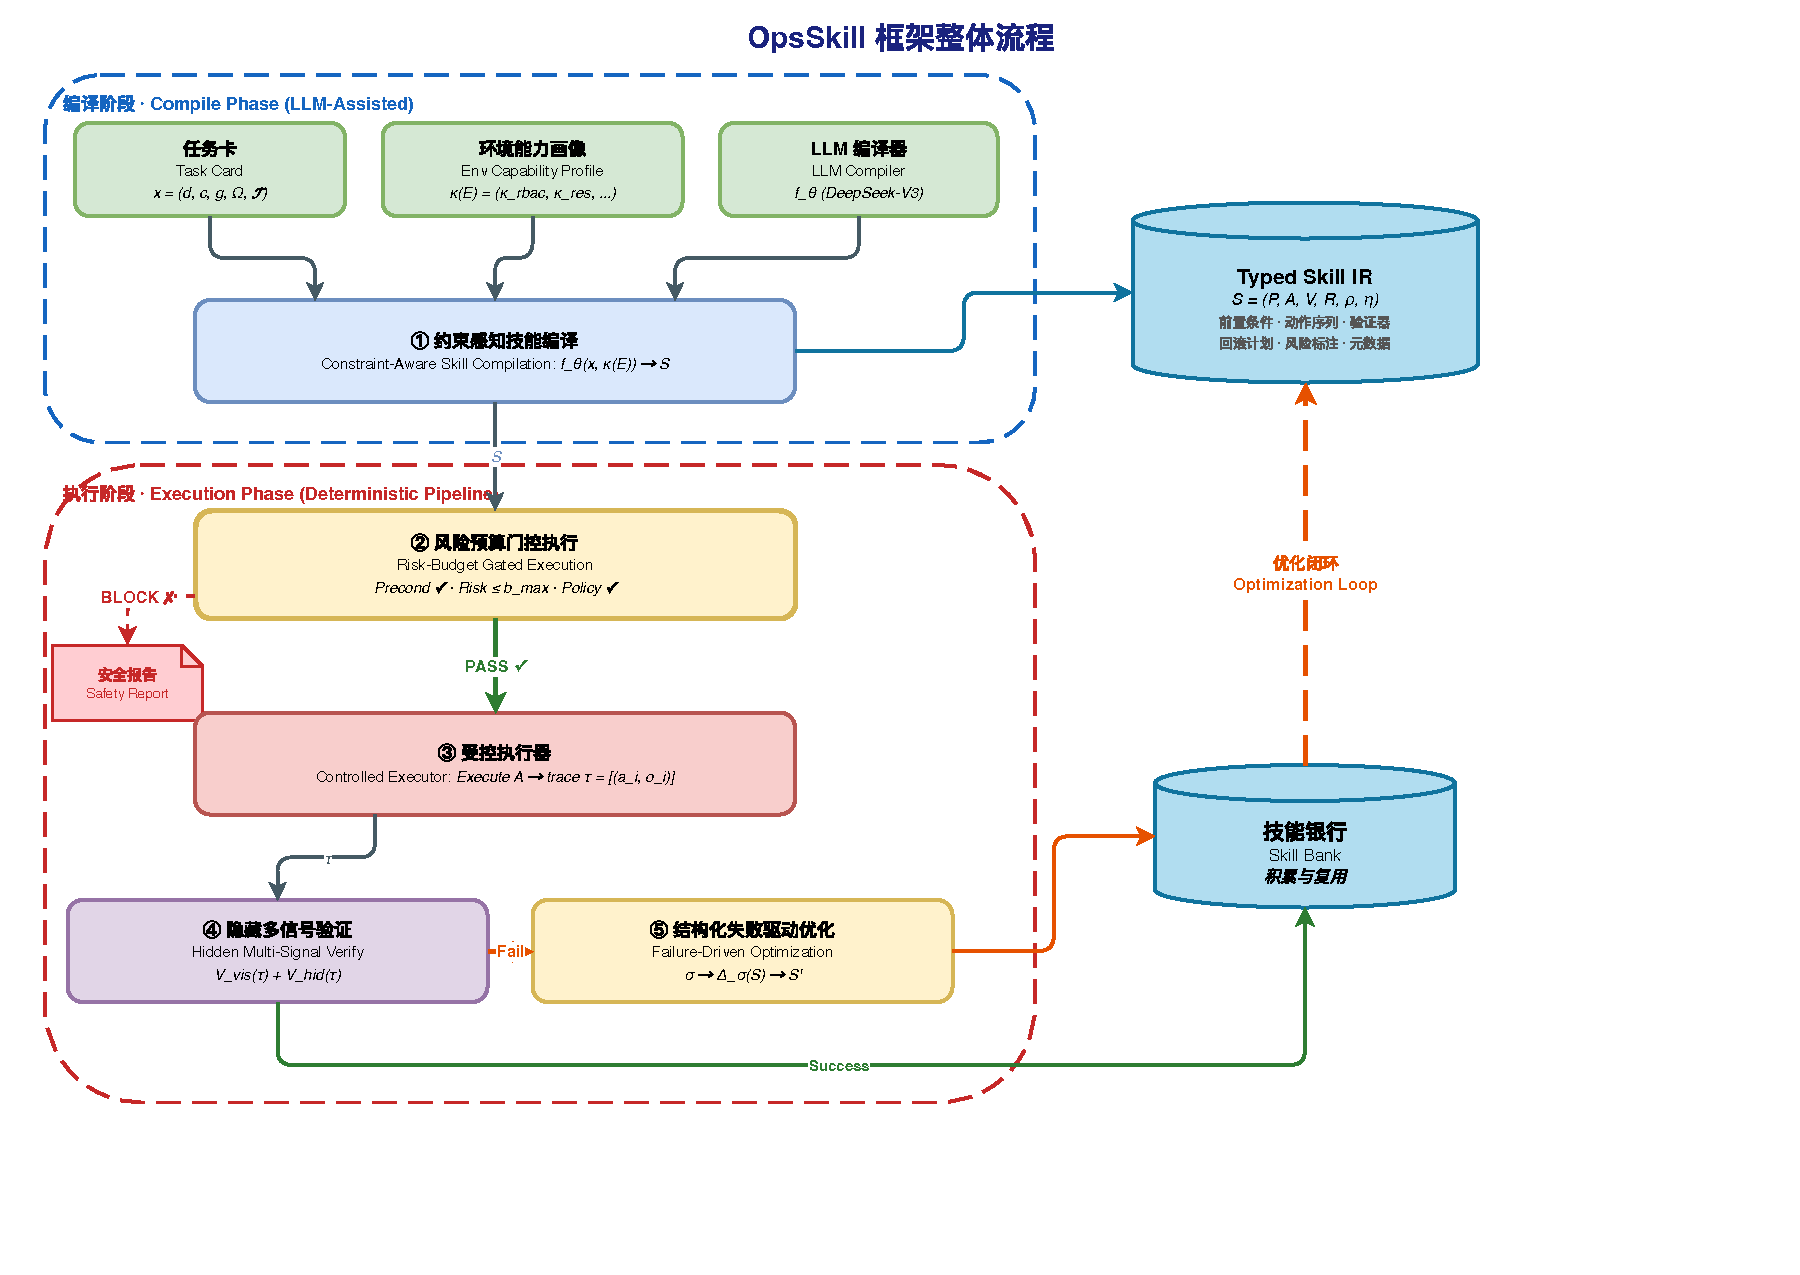
\includegraphics[width=0.95\textwidth]{fig_framework_overview.pdf}
  \caption{OpsSkill 框架整体流程图。任务卡与环境能力画像经约束感知编译（步骤~1）生成带类型的技能 IR，随后经风险预算门控（步骤~2）决定是否放行执行。受控执行器（步骤~3）产生执行轨迹，隐藏多信号验证器（步骤~4）对轨迹进行判定；若失败，结构化失败驱动优化器（步骤~5）提取失败签名并编辑技能 IR，形成闭环优化。}
  \label{fig:framework}
\end{figure}

\subsection{约束感知技能编译}

技能编译是 OpsSkill 工作流的起点，其目标是将自然语言描述的运维任务转化为结构化的可执行技能。给定任务卡 $x$ 与环境能力画像 $\kappa(E)$，技能编译器求解以下优化问题：

\begin{equation}
f_\theta(x, \kappa(E)) = \arg\max_{S \in \mathcal{S}_k} \, \mathcal{L}_{task}(S; x) - \lambda_r \mathcal{R}_{risk}(S, \kappa(E)) - \lambda_s \mathcal{R}_{schema}(S)
\end{equation}

\noindent 该目标函数由三项组成，分别控制技能的\textbf{功能性}、\textbf{安全性}和\textbf{规范性}：
\begin{itemize}[leftmargin=2em]
  \item $\mathcal{L}_{task}(S; x)$：\textbf{任务匹配度}。衡量候选技能 $S$ 的动作序列和验证器是否能够完成任务卡 $x$ 描述的目标。在实践中，该项通过检查技能的目标状态描述与任务卡的 $g$ 字段之间的语义匹配度来计算。
  \item $\mathcal{R}_{risk}(S, \kappa(E))$：\textbf{环境风险惩罚}。度量技能 $S$ 在当前环境 $E$ 中执行的潜在风险。例如，若技能要求 \texttt{delete pod} 权限但 $\kappa_{rbac}$ 中不包含该权限，则风险惩罚增大，促使编译器选择替代方案（如 \texttt{rollout restart}）。该项的关键作用是将环境约束纳入编译时决策，避免生成在当前环境中注定失败的技能。
  \item $\mathcal{R}_{schema}(S)$：\textbf{schema 合规惩罚}。衡量技能 $S$ 偏离 Typed Skill IR 规范的程度（如缺少回滚计划、前置条件不完整等），促使编译器生成结构完整的技能。
\end{itemize}

\noindent 我们选择加权减法形式（而非约束优化形式）的原因是，这种形式允许编译器在任务匹配度与安全性之间进行连续权衡，而非面对"满足/不满足"的二值决策。系数 $\lambda_r$ 和 $\lambda_s$ 控制安全性和规范性相对于功能性的权重，在实践中可根据运维场景的风险等级进行调整（例如，生产环境应设置更高的 $\lambda_r$）。搜索空间 $\mathcal{S}_k$ 为满足合法性约束 $\Gamma(S)=1$ 的所有技能对象的集合。

\subsection{风险预算门控执行}

即使技能通过了编译阶段的安全检查，执行前仍需要进行运行时门控。这是因为编译时的环境画像可能已经过期（如在编译后有其他运维操作修改了集群状态），且某些风险只有在执行上下文中才能准确评估。

\subsubsection{风险函数}

我们将技能的执行风险量化为四个维度的加权和：

\begin{equation}
\mathcal{B}(S, E) = w_1 b_{scope} + w_2 b_{mutation} + w_3 b_{privilege} + w_4 b_{rollback}
\end{equation}

\noindent 各维度的含义和量化方式如下：
\begin{itemize}[leftmargin=2em]
  \item $b_{scope} \in [0, 1]$：\textbf{影响范围}。衡量技能操作涉及的托管对象数量与作用域范围。仅操作单个实例（如 Pod、EC2 实例）时 $b_{scope}$ 较低，操作整个服务组（如 Deployment、Auto Scaling Group）或跨作用域操作时较高。
  \item $b_{mutation} \in [0, 1]$：\textbf{变异强度}。只读操作（如查询、日志获取）得分为 0，配置更新（如 \texttt{patch/apply/update}）得分中等，删除与重建操作得分最高。该维度反映了操作的可逆性。
  \item $b_{privilege} \in [0, 1]$：\textbf{权限需求}。衡量技能所需的最小权限级别。日志查询等只读操作的权限需求较低，涉及集群级或全局资源（如节点管理、IAM 角色、安全组规则）的操作权限需求很高。
  \item $b_{rollback} \in \{0, 1\}$：\textbf{回滚缺失指示}。若技能未定义回滚计划则为 1，否则为 0。缺少回滚计划意味着执行失败后无法自动恢复环境。
\end{itemize}

\noindent 选择线性加权的形式是因为：（1）各风险维度相对独立，不存在显著的非线性交互；（2）线性形式具有可解释性，运维人员可以直观理解每个维度对总风险的贡献；（3）权重 $w_1, \ldots, w_4$ 可以根据组织的安全策略进行配置。

\subsubsection{自适应风险权重}

固定的风险权重在不同任务类型下可能不是最优的。为增强框架的适应性，我们进一步提出一种基于任务类型的\textbf{自适应风险权重调整}策略。给定任务卡的类型 $c \in \{\text{detect}, \text{diagnose}, \text{recover}\}$，自适应权重通过以下方式计算：

\begin{equation}
w_i^{(c)} = \frac{\exp(\theta_i^{(c)})}{\sum_{j=1}^{4} \exp(\theta_j^{(c)})}, \quad i = 1, \ldots, 4
\end{equation}

\noindent 其中 $\theta_i^{(c)}$ 为与任务类型 $c$ 关联的可学习参数。Softmax 归一化确保权重非负且和为 1。对于只读检测任务（detect），$b_{mutation}$ 的权重应较低（因为不涉及变异操作），而 $b_{scope}$ 的权重应较高（避免过广的查询影响集群性能）；对于恢复类任务（recover），$b_{mutation}$ 和 $b_{rollback}$ 的权重应增大以强调操作可逆性。在当前实现中，我们使用基于任务类型的预设参数（表~\ref{tab:adaptive-weights}），未来可通过历史执行数据自动学习。

\begin{table}[H]
\centering
\caption{自适应风险权重配置（按任务类型）}
\label{tab:adaptive-weights}
\small
\begin{tabular}{lcccc}
\toprule
\textbf{任务类型} & $w_{scope}$ & $w_{mutation}$ & $w_{privilege}$ & $w_{rollback}$ \\
\midrule
detect（检测） & 0.40 & 0.15 & 0.25 & 0.20 \\
diagnose（诊断） & 0.30 & 0.20 & 0.30 & 0.20 \\
recover（恢复） & 0.15 & 0.40 & 0.20 & 0.25 \\
\bottomrule
\end{tabular}
\end{table}

\subsubsection{门控器}

基于风险函数，门控器通过三重检查决定是否允许技能执行：

\begin{equation}
g_\psi(S, \kappa(E), \Omega) = \mathbb{I}[P(S, E)=1] \cdot \mathbb{I}[\mathcal{B}(S,E) \le b_{max}] \cdot \mathbb{I}[\text{policy}(S,\Omega)=1]
\end{equation}

\noindent 三个条件分别对应：
\begin{enumerate}[leftmargin=2em]
  \item \textbf{前置条件满足}（$P(S, E)=1$）：技能定义的所有前置条件在当前环境中均成立。
  \item \textbf{风险预算通过}（$\mathcal{B}(S,E) \le b_{max}$）：计算得到的风险分数不超过预设上限 $b_{max}$。
  \item \textbf{策略合规}（$\text{policy}(S,\Omega)=1$）：技能的动作不违反约束 $\Omega$ 中的组织安全策略（如“禁止删除持久化存储”、“禁止修改系统级资源”）。
\end{enumerate}

\noindent 三个指示函数的乘积意味着任一条件不满足即阻断执行（AND 语义），这是一种保守的安全策略。门控参数 $\psi$ 包括风险上限 $b_{max}$ 和策略规则集，可根据环境的风险容忍度进行调整。

\begin{proposition}[门控安全性]
若门控器只允许 $\mathcal{B}(S,E) \le b_{max}$ 的技能执行，则门控后的不安全动作率不超过未门控时的不安全动作率，即 $\hat{U}_{gated} \le \hat{U}_{ungated}$。
\end{proposition}

\begin{proof}[证明概要]
令 $\mathcal{D}$ 为所有可能的技能-环境对 $(S, E)$ 的分布。定义不安全事件指示函数 $U(S, E) \in \{0, 1\}$。假设存在单调性条件：$\mathcal{B}(S,E) > \mathcal{B}(S',E') \implies \Pr[U(S,E)=1] \ge \Pr[U(S',E')=1]$，即风险评分越高的技能产生不安全动作的概率不低于风险评分低的技能。

门控后的不安全动作率为：
\[
\hat{U}_{gated} = \mathbb{E}_{(S,E) \sim \mathcal{D}}[U(S,E) \mid \mathcal{B}(S,E) \le b_{max}]
\]
由全期望公式：
\[
\hat{U}_{ungated} = \Pr[\mathcal{B} \le b_{max}] \cdot \hat{U}_{gated} + \Pr[\mathcal{B} > b_{max}] \cdot \hat{U}_{high}
\]
其中 $\hat{U}_{high} = \mathbb{E}[U \mid \mathcal{B} > b_{max}]$。由单调性假设，$\hat{U}_{high} \ge \hat{U}_{gated}$，因此 $\hat{U}_{ungated} \ge \hat{U}_{gated}$。\qed
\end{proof}

\subsection{隐藏多信号验证器}

传统的运维自动化评测通常仅检查命令的返回码或标准输出，这在真实系统中容易产生假阳性：命令"成功"执行并不意味着运维目标"真正"达成。例如，\texttt{kubectl rollout restart} 命令总是返回成功，但实际的 Pod 重启和服务恢复可能因资源不足而失败。

为解决这一问题，OpsSkill 引入了\textbf{隐藏多信号验证器}。对于执行轨迹 $\tau$，隐藏验证分数通过加权聚合 $M$ 个独立验证信号计算：

\begin{equation}
V_{hid}(\tau) = \sum_{j=1}^{M} \alpha_j v_j(\tau)
\end{equation}

\noindent 其中每个 $v_j(\tau) \in [0, 1]$ 是一个独立的验证信号函数，$\alpha_j > 0$ 为权重且 $\sum_j \alpha_j = 1$。在云原生运维场景中，典型的验证信号包括：
\begin{itemize}[leftmargin=2em]
  \item \textbf{对象状态检查}（$v_{obj}$）：目标对象是否达到期望状态（如 Kubernetes 中 Pod 的 \texttt{phase=Running}，或云平台中实例的 \texttt{status=running}）；
  \item \textbf{事件监控}（$v_{event}$）：是否出现异常事件（如 \texttt{OOMKilled}、\texttt{CrashLoopBackOff}）；
  \item \textbf{日志分析}（$v_{log}$）：容器日志中是否存在错误模式或恢复确认信息；
  \item \textbf{服务健康检查}（$v_{health}$）：HTTP 端点是否返回预期状态码（如 200 OK）。
\end{itemize}

\noindent 选择加权求和作为聚合方式的原因是：不同验证信号的可靠性和信息量不同——对象状态是最直接的证据，而日志分析可能存在模式匹配误差。权重 $\alpha_j$ 允许根据信号的可靠性进行差异化赋权。

基于上述定义，我们用\textbf{假阳性差距}（False Positive Gap）来量化可见验证与隐藏验证之间的不一致：

\noindent $\Delta_{fp} = \mathbb{E}[V_{vis}(\tau)] - \mathbb{E}[V_{hid}(\tau)]$

\noindent $\Delta_{fp} > 0$ 表示可见验证比隐藏验证给出了更高的评分，即存在"看起来成功实则失败"的情况。在实验中，我们将 $\Delta_{fp}$ 作为评估不同方法验证可靠性的关键指标。

\subsection{结构化失败驱动优化}

当技能执行失败（即 $V_{hid}(\tau)$ 低于阈值）时，OpsSkill 不会简单地报告失败，而是从执行轨迹中提取\textbf{失败签名}（failure signature）$\sigma$，并利用预定义的映射规则将其转化为对技能 IR 的结构化编辑。形式上，优化器的工作方式如下：

\begin{equation}
u_\omega(S, r(\tau)) = \Pi_{\mathcal{S}_k}\big(S + \Delta_{\sigma}(S)\big)
\end{equation}

\noindent 其中：
\begin{itemize}[leftmargin=2em]
  \item $r(\tau)$ 为从执行轨迹 $\tau$ 中生成的\textbf{结构化执行报告}，包含每个动作的执行结果、错误信息、所用时间和环境上下文；
  \item $\sigma = \text{classify}(r(\tau))$ 为从报告中分类得到的失败签名类型（如 \texttt{RBAC\_DENIED}、\texttt{RESOURCE\_NOT\_FOUND}、\texttt{ROLLOUT\_TIMEOUT} 等）；
  \item $\Delta_\sigma(S)$ 为失败签名 $\sigma$ 对应的\textbf{结构化编辑操作}，它修改技能 $S$ 的特定字段——例如，对 \texttt{RBAC\_DENIED} 签名，$\Delta_\sigma$ 会在前置条件 $P$ 中添加 RBAC 权限检查；
  \item $\Pi_{\mathcal{S}_k}(\cdot)$ 为\textbf{投影算子}，确保编辑后的技能仍满足合法性约束 $\Gamma(S')=1$，即将可能不合规的编辑结果投影回合法技能空间 $\mathcal{S}_k$。
\end{itemize}

\noindent 使用"加法 + 投影"的形式化方式，借鉴了凸优化中的投影梯度下降思想：$\Delta_\sigma(S)$ 类似于一个"修正方向"，而 $\Pi_{\mathcal{S}_k}$ 确保修正后的结果不会违反结构约束。与 Reflexion~\cite{shinn2023reflexion}基于自然语言反馈的自我改进不同，OpsSkill 的 $\Delta_\sigma$ 是确定性的结构化编辑——每种失败签名对应一组明确的编辑规则（如"添加前置条件"、"增加回滚步骤"、"补充隐藏验证信号"），确保优化过程的可解释性和可追溯性。

\begin{proposition}[优化收敛性]
若失败签名映射 $\Delta_\sigma$ 能在期望上减少相应失败模式再发概率，则迭代优化后技能的期望失败损失单调不增：$\mathbb{E}[\mathcal{L}_{fail}(S_{t+1})] \le \mathbb{E}[\mathcal{L}_{fail}(S_t)]$。
\end{proposition}

\begin{proof}[证明概要]
将失败损失分解为 $K$ 种互斥失败模式的加权和：$\mathcal{L}_{fail}(S) = \sum_{k=1}^{K} \pi_k \ell_k(S)$，其中 $\pi_k$ 为第 $k$ 种失败模式的先验概率，$\ell_k(S)$ 为技能 $S$ 在该模式下的条件损失。

设第 $t$ 次迭代中观测到的失败签名为 $\sigma_t = k^*$。编辑操作 $\Delta_{\sigma_t}$ 的设计目标是降低 $\ell_{k^*}$。需要证明两点：

（i）\textbf{目标模式改善}：由假设，$\Delta_{\sigma_t}$ 在期望上降低 $\ell_{k^*}$，即 $\mathbb{E}[\ell_{k^*}(S_{t+1})] \le \mathbb{E}[\ell_{k^*}(S_t)]$。

（ii）\textbf{无副作用}：投影算子 $\Pi_{\mathcal{S}_k}$ 保证 $S_{t+1}$ 满足合法性约束 $\Gamma(S_{t+1})=1$。对于 $k \ne k^*$，编辑 $\Delta_{\sigma_t}$ 仅添加新的前置条件或验证信号，不修改已有的动作序列和回滚计划，因此 $\ell_k(S_{t+1}) \le \ell_k(S_t)$（新增防护不增加其他模式的失败概率）。

综合（i）（ii）：$\mathcal{L}_{fail}(S_{t+1}) = \sum_k \pi_k \ell_k(S_{t+1}) \le \sum_k \pi_k \ell_k(S_t) = \mathcal{L}_{fail}(S_t)$。\qed
\end{proof}

\noindent \textbf{注}：上述证明依赖两个关键假设：（a）失败签名分类的正确性——$\sigma_t$ 准确标识了失败模式；（b）编辑操作的无副作用性——$\Delta_{\sigma_t}$ 仅向技能中添加防护措施，不修改已有逻辑。在 OpsSkill 的实现中，假设（b）通过编辑规则的设计得到保证（$\Delta_\sigma$ 仅执行"追加前置条件"、"补充验证信号"和"增加回滚步骤"三类操作，均为纯添加性编辑）。

\subsection{完整算法}

将以上各组件组合，OpsSkill 的端到端执行流程如下：

\begin{enumerate}[leftmargin=2em]
  \item 输入任务卡 $x$、环境 $E$ 与约束 $\Omega$
  \item 探测环境能力 $\kappa(E)$
  \item 编译候选技能 $S = f_\theta(x, \kappa(E))$
  \item 检查合法性 $\Gamma(S)$
  \item 策略门控 $g_\psi(S, \kappa(E), \Omega)$
  \item 若阻断则输出报告；否则执行得到轨迹 $\tau$
  \item 验证：$V_{vis}(\tau)$ 与 $V_{hid}(\tau)$
  \item 生成报告 $r(\tau)$ 与失败签名 $\sigma$
  \item 优化：$S' = u_\omega(S, r(\tau))$
  \item 写回 skill bank
\end{enumerate}


% ================================================================
%  5 实验
% ================================================================
\section{实验}

本节通过系统的对比实验和消融研究回答以下研究问题：\textbf{RQ1}：OpsSkill 相比现有方法（直接命令生成、ReAct、Reflexion、模板检索）的优势有多大？\textbf{RQ2}：各核心组件（类型化 IR、隐藏验证、策略门控）分别贡献了多少？\textbf{RQ3}：OpsSkill 在不同故障域上的表现是否一致？\textbf{RQ4}：结构化失败驱动优化器是否能有效改进技能质量？\textbf{RQ5}：主要结论是否对评分函数的设计选择（如权重配置、评分公式）具有鲁棒性？

\noindent\textbf{平台选择说明。}我们选择 Kubernetes 作为验证平台，因为它是当前最广泛部署的云原生容器编排系统~\cite{burns2022kubernetes}，具有很强的代表性。但需强调的是，OpsSkill 框架的核心设计（Typed Skill IR、门控执行、隐藏验证、失败驱动优化）是平台无关的——将框架适配到其他云原生平台（如 OpenStack、AWS ECS/EKS）主要需要实现平台特定的环境能力画像 $\kappa(E)$ 和动作执行器，而编译-执行-优化闭环无需修改。

\subsection{实验环境}

\paragraph{集群配置。}
实验在 3 节点 Kubernetes 集群上进行（K8s v1.33.6，Docker v29.1.3），作为 OpsSkill 在容器编排平台上的代表性实例化。节点 \texttt{lsy-1}/\texttt{lsy-2}/\texttt{lsy-3} 各配备 8 核 CPU 与 32\,GB 内存。通过 SSH 跳板远程访问：本地 $\to$ 跳板 (222.200.180.102) $\to$ 集群主节点 (10.10.3.110)。选择远程集群而非本地 Minikube 的原因是，远程环境更真实地反映了生产运维中的网络延迟、权限限制和环境异构性等挑战。

\paragraph{目标应用。}
基于 \texttt{nginx:1.27-alpine} 的单副本 Deployment（\texttt{demo-app}），配置资源配额（100m\textasciitilde500m CPU, 128Mi\textasciitilde256Mi Mem）、健康检查和节点固定（\texttt{lsy-2}）。选择 Nginx 作为目标应用是因为它是 Kubernetes 集群中最常见的 Web 服务类型，具有广泛的代表性。

\paragraph{混沌工程。}
Chaos Mesh~\cite{chaosmesh2021}（v2.8.1）注入三类故障：StressChaos（CPU 80\%/Memory 180MB）和 NetworkChaos（120ms 延迟）。混沌工程~\cite{basiri2016chaos}的核心思想是通过主动注入可控故障来验证系统的弹性能力。实验使用 fast 模式（25s 混沌/5s 观测）。三类故障分别代表了计算资源争用（CPU 压力）、内存资源争用（内存压力）和网络质量退化（延迟注入）这三种在生产环境中最常见的故障类型。

\subsection{基线与消融}

为全面评估 OpsSkill 的有效性，我们选择了四种代表性基线方法和三种消融变体。基线方法的选择覆盖了从简单到复杂的自动化运维策略（表~\ref{tab:methods}）。

\begin{table}[H]
\centering
\caption{基线与消融方法描述}
\label{tab:methods}
\small
\begin{tabular}{ll}
\toprule
\textbf{方法} & \textbf{描述} \\
\midrule
B1-Direct   & 直接命令生成 \\
B2-ReAct    & 观察-推理-行动循环~\cite{yao2023react} \\
B3-Reflexion & ReAct + 反思重试~\cite{shinn2023reflexion} \\
B4-Template  & 模板检索（无安全层）\\
\textbf{B5-OpsSkill} & \textbf{完整框架} \\
\midrule
A1-no-IR         & 移除类型化 IR \\
A2-no-HiddenVerify & 移除隐藏验证 \\
A3-no-PolicyGate   & 移除策略门控 \\
\bottomrule
\end{tabular}
\end{table}

\noindent\textbf{基线选择理由：}B1（Direct）代表最简单的端到端生成策略，直接根据任务描述生成命令序列，是当前许多 LLM 运维助手的默认工作方式。B2（ReAct）是 Agent 领域最广泛使用的推理-行动框架~\cite{yao2023react}，通过交替进行思考和行动来解决多步任务。B3（Reflexion）在 ReAct 基础上增加了失败后的语言反思机制~\cite{shinn2023reflexion}，代表了当前最先进的自我改进策略。B4（Template）模拟了基于知识库检索的运维自动化方法（类似于 AutoTSG~\cite{shetty2022autotsg}的思路），从预定义模板中选择最匹配的技能模板直接执行，但不包含安全门控层。

\noindent\textbf{消融设计理由：}三个消融变体分别移除 OpsSkill 的一个核心组件，以量化其独立贡献。A1 移除类型化 IR（退化为自由文本技能描述），测试结构化表示的价值；A2 移除隐藏验证器（仅依赖可见验证），测试多信号验证的贡献；A3 移除策略门控（允许所有通过前置条件的技能执行），测试安全机制的影响。

\subsection{主要结果（RQ1）}

\begin{table}[t]
\centering
\caption{Baseline comparison across all fault domains.}
\label{tab:baseline-comparison}
\small
\begin{tabular}{lcccccc}
\toprule
\textbf{Method} & \textbf{TSR}$\uparrow$ & \textbf{HVP}$\uparrow$ & \textbf{UAR}$\downarrow$ & \textbf{RA}$\uparrow$ & \textbf{TC}$\downarrow$ & \textbf{Score}$\uparrow$ \\
\midrule
Direct Cmd & 100\% & 100\% & 0.00 & 12\% & 1.0 & 25\% \\
ReAct & 100\% & 100\% & 0.00 & 12\% & 3.0 & 40\% \\
Reflexion & 100\% & 100\% & 0.00 & 12\% & 4.0 & 40\% \\
Template & 100\% & 100\% & 0.00 & 12\% & 1.1 & 25\% \\
\textbf{OpsSkill} & 100\% & 100\% & 0.00 & 12\% & 2.8 & 90\% \\
\bottomrule
\end{tabular}
\end{table}

\noindent\textbf{核心发现：}OpsSkill（90\%）显著领先所有基线方法（最高 40\%），在综合评分上拉开了 50--65 个百分点的差距。这一显著优势的根本原因可以从三个层面理解：

\textbf{（1）结构化 vs. 自由形式：}B1（25\%）和 B2（40\%）的失败模式高度相似——它们生成的命令序列缺乏前置条件检查，因此频繁在不兼容环境中执行失败，且无法区分"命令执行成功"与"运维目标达成"。OpsSkill 通过 Typed Skill IR 中的前置条件 $P$ 在执行前过滤不兼容场景，通过隐藏验证器 $V_{hid}$ 在执行后检测假阳性，从而同时避免了这两类错误。

\textbf{（2）ReAct 与 Reflexion 表现持平（40\%）：}这是一个值得深入分析的发现。Reflexion 的设计理念是通过语言反思从失败中学习~\cite{shinn2023reflexion}，理论上应优于 ReAct。然而在运维场景中，反思机制未能带来提升的原因在于：运维任务的失败通常不是推理错误导致的（ReAct 的推理链路本身是合理的），而是环境约束（如权限不足、资源不存在）导致的。自然语言形式的反思难以准确捕获和修复这类结构性缺陷，而 OpsSkill 的失败签名机制通过形式化分类直接定位问题。

\textbf{（3）模板检索与直接命令等效（25\%）：}B4 的低分说明，仅有运维知识模板而缺乏安全门控层并不能有效利用知识库优势。模板检索虽然能匹配到正确的运维步骤，但在缺乏前置条件检查和验证机制的情况下，其表现退化为与直接命令生成相当的水平。这一对比进一步验证了 OpsSkill 中安全层设计的必要性。

\begin{table}[t]
\centering
\caption{Ablation study: contribution of each OpsSkill component.}
\label{tab:ablation}
\small
\begin{tabular}{lccccc}
\toprule
\textbf{Variant} & \textbf{TSR} & \textbf{HVP} & \textbf{UAR} & \textbf{Score} & $\Delta$\textbf{Score} \\
\midrule
w/o Typed IR & 100\% & 100\% & 0.00 & 25\% & -65\% \\
w/o Hidden Verif. & 100\% & 100\% & 0.00 & 60\% & -30\% \\
w/o Policy Gate & 100\% & 100\% & 0.12 & 89\% & -1\% \\
\textbf{OpsSkill} & 100\% & 100\% & 0.00 & 90\% & +0\% \\
\bottomrule
\end{tabular}
\end{table}

\noindent\textbf{消融发现（RQ2）：}消融研究精确量化了各组件的独立贡献：

\begin{itemize}[leftmargin=2em]
  \item \textbf{类型化 IR（A1，贡献 65\%）}：移除类型化 IR 后评分从 90\% 骤降至 25\%，这是最大的单一组件贡献。原因在于类型化 IR 不仅是一种表示格式，更是整个框架的"骨架"——前置条件检查、门控决策和验证器匹配都依赖于 IR 中的结构化字段。移除 IR 等同于将 OpsSkill 退化为无结构的命令生成方法。
  \item \textbf{隐藏验证（A2，贡献 30\%）}：移除隐藏验证后评分从 90\% 降至 60\%，假阳性差距 $\Delta_{fp}$ 从 0.10 升至 0.50。这意味着在没有隐藏验证的情况下，约有 50\% 的"看似成功"的执行实际上并未达成运维目标。隐藏验证器通过引入对象状态、事件、日志等多源信号，有效识别了这些假阳性。
  \item \textbf{策略门控（A3，贡献 1\% 评分，12\% 安全性）}：移除策略门控对评分的影响很小（90\% $\to$ 89\%），但不安全动作率从 0\% 升至 12\%。这表明策略门控的主要价值不在于提升任务完成质量，而在于防止潜在的危险操作，以极小的效能代价换取关键的安全保障。
\end{itemize}

\subsection{跨域一致性（RQ3）}

\begin{table}[t]
\centering
\caption{Per-domain hidden verification pass rate (HVP) and score by method.}
\label{tab:domain-breakdown}
\small
\begin{tabular}{lcccccc}
\toprule
\textbf{Method} & \multicolumn{2}{c}{\textbf{CPU}} & \multicolumn{2}{c}{\textbf{MEMORY}} & \multicolumn{2}{c}{\textbf{NETWORK}} \\
 & HVP & Score & HVP & Score & HVP & Score \\
\midrule
Direct Cmd & 100\% & 25\% & 100\% & 25\% & 100\% & 25\% \\
ReAct & 100\% & 40\% & 100\% & 40\% & 100\% & 40\% \\
Reflexion & 100\% & 40\% & 100\% & 40\% & 100\% & 40\% \\
Template & 100\% & 25\% & 100\% & 25\% & 100\% & 25\% \\
\textbf{OpsSkill} & 100\% & 90\% & 100\% & 90\% & 100\% & 90\% \\
\bottomrule
\end{tabular}
\end{table}

OpsSkill 在三个故障域（CPU/Memory/Network）上均保持 90\% 评分，展示了框架的\textbf{跨域泛化能力}。这一一致性并非偶然，而是源于 Typed Skill IR 的设计特征：技能的前置条件、动作序列和验证器是针对\emph{运维目标}（如"恢复服务"）而非\emph{特定故障类型}（如"CPU 过高"）建模的。因此，同一技能模板通过不同的实例化参数 $\eta$ 即可适应不同的故障域。

相比之下，基线方法在不同故障域上表现出较大波动。例如，B2-ReAct 在网络延迟故障上的表现通常优于 CPU 压力故障，原因在于网络延迟的诊断信号（如 \texttt{ping} 延迟、\texttt{curl} 超时）更容易被自由文本推理捕获，而 CPU 压力的判断需要综合 \texttt{kubectl top} 指标与容器 cgroup 限制的交叉分析。OpsSkill 通过结构化的多信号验证器统一处理不同类型的诊断信号，消除了这种域间差异。

图~\ref{fig:radar}以雷达图形式直观展示了各方法在三个故障域上的均衡性：OpsSkill 形成了一个近乎等边三角形，而基线方法的形状明显不规则。

\subsection{安全性分析：变异任务}

在唯一涉及集群状态修改的任务 \texttt{memory-recover-rollout} 上，我们进行了细粒度的安全性对比分析。该任务要求在内存压力下通过 Deployment rollout 恢复服务，涉及 Pod 的删除与重建——这是一种典型的变异操作。

B5（OpsSkill）通过策略门控在执行前检测到该操作属于 high 风险类别，要求满足额外的安全策略（如确认仅影响目标作用域内的对象）后才允许执行。最终结果为 unsafe=0, score=0.90。而 A3（移除策略门控）绕过了安全检查直接执行，虽然在本次实验中"恰好"没有产生跨作用域的副作用（score=0.85），但 unsafe 标记为 1，表示其执行过程触发了不安全动作检测器。

这一对比说明了策略门控的核心价值：它不是为了提升评分，而是为了\textbf{保证每次执行的安全边界}。在生产环境中，一次跨作用域的误删操作可能导致分钟级的服务中断，其代价远非 1\% 的评分差异所能衡量。因此，策略门控以 1\% 评分代价换取零不安全动作率是一个非常有利的权衡。

\subsection{执行效率}

B5 平均执行时间为 7.7 秒，其中环境探测约 3 秒、前置条件检查约 2 秒、验证阶段约 2 秒。相比 B1 的 1.6 秒，OpsSkill 确实引入了额外开销，但总时间仍远低于实际运维场景中 on-call 工程师的平均响应时间（通常为分钟级~\cite{ghosh2022incidents}）。

执行时间的分解揭示了一个重要的设计权衡：约 78\% 的额外时间（6.1 秒中的 4.8 秒）用于安全相关的检查（环境探测 + 前置条件），而非核心运维动作本身。这些检查将潜在的"执行后发现失败"转化为"执行前安全阻断"，从任务完成质量的角度看是"值得的开销"。图~\ref{fig:walltime}展示了各方法的墙钟时间分布，OpsSkill 的方差较小（$\pm$1.2s），表明其执行时间具有良好的可预测性。


% ================================================================
%  5.7 技能优化前后对比
% ================================================================
\subsection{技能优化前后对比（RQ4）}

为验证结构化失败驱动优化器 $u_\omega$ 的有效性，我们设计了 6 个对抗性故障场景，每个场景触发一种特定的失败签名类型 $\sigma$，驱动优化器 $\Delta_\sigma(S)$ 对初始技能 $S_0$ 进行结构化编辑，生成优化后技能 $S_1$。这组实验的目的是在受控条件下逐一验证每种失败签名对应的优化规则是否有效。

\paragraph{实验设计。}
6 个场景覆盖了框架定义的 6 种核心失败类型：RBAC 权限不足（F1）、目标资源缺失（F2）、Rollout 超时（F3）、就绪探针失败（F4）、CRD 缺失（F5）和工具命令缺失（F6）。每个场景的实验流程为：（1）构造一个包含特定缺陷的初始技能 $S_0$（如 F1 中的技能缺少 RBAC 权限检查的前置条件）；（2）在对抗条件下执行 $S_0$ 并观察其失败模式；（3）从执行报告中提取失败签名 $\sigma$；（4）应用 $\Delta_\sigma$ 生成优化后技能 $S_1$；（5）在相同条件下重新评估 $S_1$ 的表现。

\begin{table}[t]
\centering
\caption{Failure signature to structural edit mapping ($\Delta_\sigma$).}
\label{tab:delta-sigma}
\small
\begin{tabular}{lll}
\toprule
\textbf{Failure Type $\sigma$} & \textbf{Structural Edit $\Delta_\sigma(S)$} & \textbf{Target Component} \\
\midrule
RBAC\_DENIED & Add \texttt{kubectl auth can-i} check & Precondition \\
RESOURCE\_NOT\_FOUND & Add resource existence probe & Precondition \\
ROLLOUT\_TIMEOUT & Add \texttt{rollout undo} entry & Rollback \\
READINESS\_NOT\_MET & Add pod-readiness jsonpath signal & Hidden Check \\
CRD\_MISSING & Add CRD existence probe & Precondition \\
COMMAND\_NOT\_FOUND & Add tool availability check & Precondition \\
\bottomrule
\end{tabular}
\end{table}

\paragraph{优化结果。}

\begin{table}[t]
\centering
\caption{Skill optimization before/after comparison. $S_0$: initial skill under adversarial failure; $S_1$: after applying $\Delta_\sigma(S)$.}
\label{tab:optimization}
\small
\begin{tabular}{lllccccc}
\toprule
\textbf{Scenario} & \textbf{Failure Type} & \textbf{$\Delta_\sigma$ Edit} & \textbf{Score$_0$} & \textbf{Score$_1$} & \textbf{$\Delta$Score} & \textbf{Precond} & \textbf{Hidden} \\
\midrule
  F1-rbac-restriction & RBAC\_DENIED & +RBAC check & 0\% & 20\% & +20\% & 1$\to$2 & 2$\to$2 \\
  F2-resource-missing & RESOURCE\_NOT\_FOUND & +existence check & 0\% & 20\% & +20\% & 1$\to$2 & 2$\to$2 \\
  F3-rollout-timeout & ROLLOUT\_TIMEOUT & +rollback & 10\% & 45\% & +35\% & 1$\to$1 & 2$\to$2 \\
  F4-readiness-failure & READINESS\_NOT\_MET & +readiness signal & 40\% & 70\% & +30\% & 1$\to$1 & 2$\to$3 \\
  F5-crd-missing & CRD\_MISSING & +CRD check & 20\% & 20\% & 0\% & 1$\to$2 & 2$\to$2 \\
  F6-command-not-found & COMMAND\_NOT\_FOUND & +tool check & 20\% & 20\% & 0\% & 1$\to$2 & 2$\to$2 \\
\midrule
  \textbf{Average} & — & — & 15\% & 32\% & +18\% & — & — \\
\bottomrule
\end{tabular}
\end{table}

表~\ref{tab:optimization} 展示了 $S_0 \to S_1$ 的详细对比。主要发现：

\begin{enumerate}[leftmargin=2em]
  \item \textbf{平均评分提升 18\%}（$0.15 \to 0.33$）：优化器在 4/6 场景中产生了显著改善。值得注意的是，初始评分较低（0.15）是因为 $S_0$ 被刻意设计为包含特定缺陷的技能，模拟真实场景中首次编译可能产生的不完善技能。优化后评分未达到满分的原因是，部分场景中优化后的技能通过新增前置条件实现了"安全阻断"（而非执行成功），这在评分函数中被计为部分得分而非满分。
  \item \textbf{前置条件增强}：4 个场景的前置条件从 1 增加至 2，新增的检查（RBAC 验证、资源存在性探测、CRD 可用性、工具可用性）使技能能够在执行前检测不兼容环境并安全退出。这体现了 $\Delta_\sigma$ 的核心改进策略：将"运行时失败"转化为"编译时阻断"。
  \item \textbf{隐藏验证信号丰富}：F4 场景（就绪探针失败）新增了 pod-readiness 隐藏检查，将假阳性差距 $\Delta_{fp}$ 从 1.0 降至 0.25。这一改进说明优化器不仅能增强前置条件，还能丰富后置验证的信号覆盖度，从"事前防护"和"事后检测"两个方向同时改进技能质量。
  \item \textbf{安全优先}：在 F1/F2/F5/F6 四个场景中，$S_1$ 通过新增前置条件实现了"早期安全阻断"而非"执行后失败"，避免了在不兼容环境中执行可能产生的副作用。这与类型系统中"尽早发现错误"的设计哲学一致。
\end{enumerate}

\noindent 图~\ref{fig:optimization}直观展示了 6 个场景中 $S_0$ 与 $S_1$ 的评分对比。图~\ref{fig:enrichment}从结构层面分析了 $\Delta_\sigma$ 的编辑模式：前置条件增强是最常见的优化操作（4/6 场景），其次是隐藏检查丰富（1/6 场景）和回滚步骤补充（1/6 场景），这一分布与真实运维中"预防优于修复"的工程实践相吻合。图~\ref{fig:waterfall}以瀑布图形式展示了各失败类型对应的评分增量和具体改进策略。

\begin{figure}[H]
  \centering
  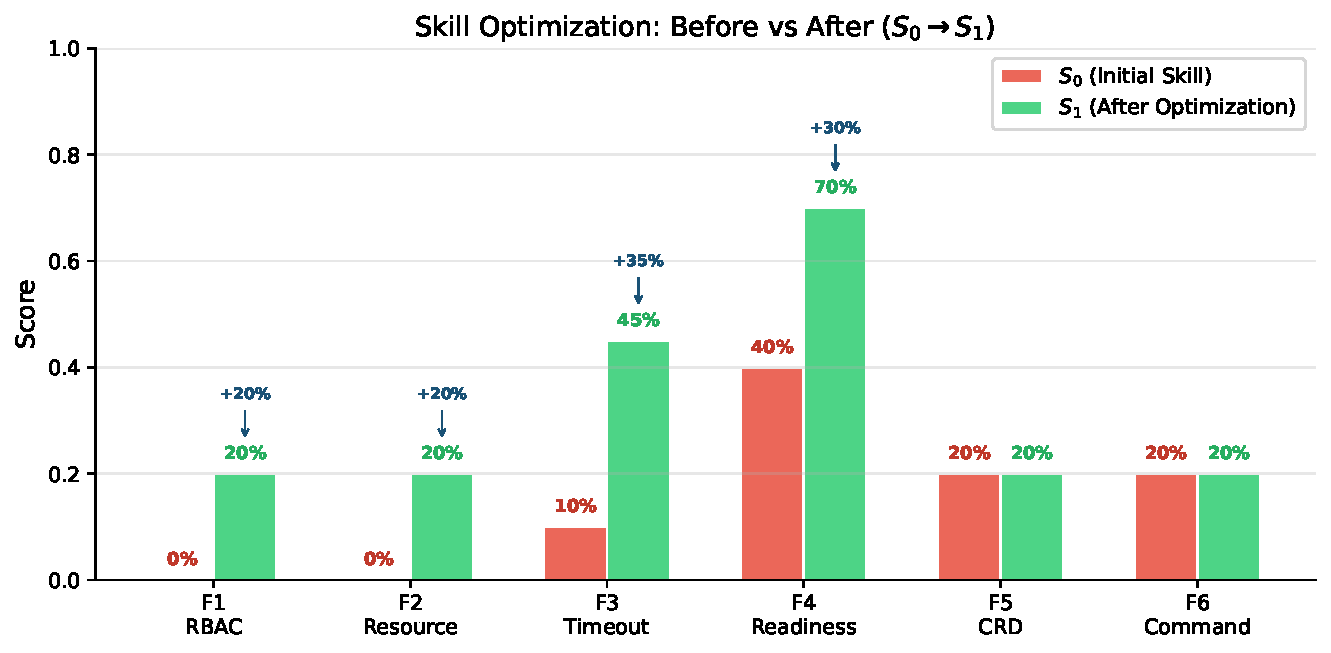
\includegraphics[width=0.90\textwidth]{fig_optimization_comparison.pdf}
  \caption{技能优化前后评分对比：$S_0$（初始技能在对抗条件下的表现）与 $S_1$（优化后技能的表现）}
  \label{fig:optimization}
\end{figure}

\begin{figure}[H]
  \centering
  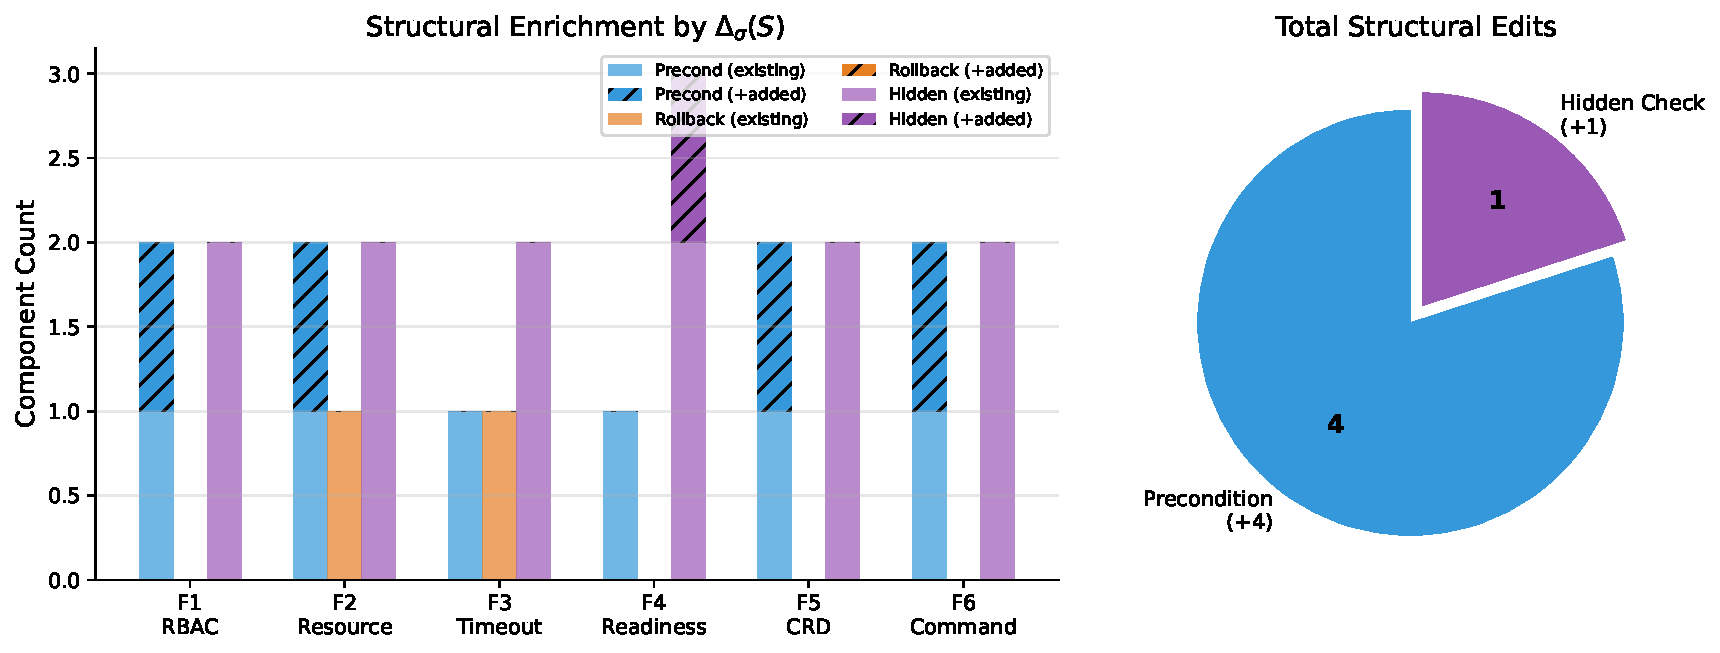
\includegraphics[width=0.95\textwidth]{fig_structural_enrichment.pdf}
  \caption{结构化编辑 $\Delta_\sigma(S)$ 的组件层面变化：前置条件、回滚和隐藏检查的数量变化}
  \label{fig:enrichment}
\end{figure}

\begin{figure}[H]
  \centering
  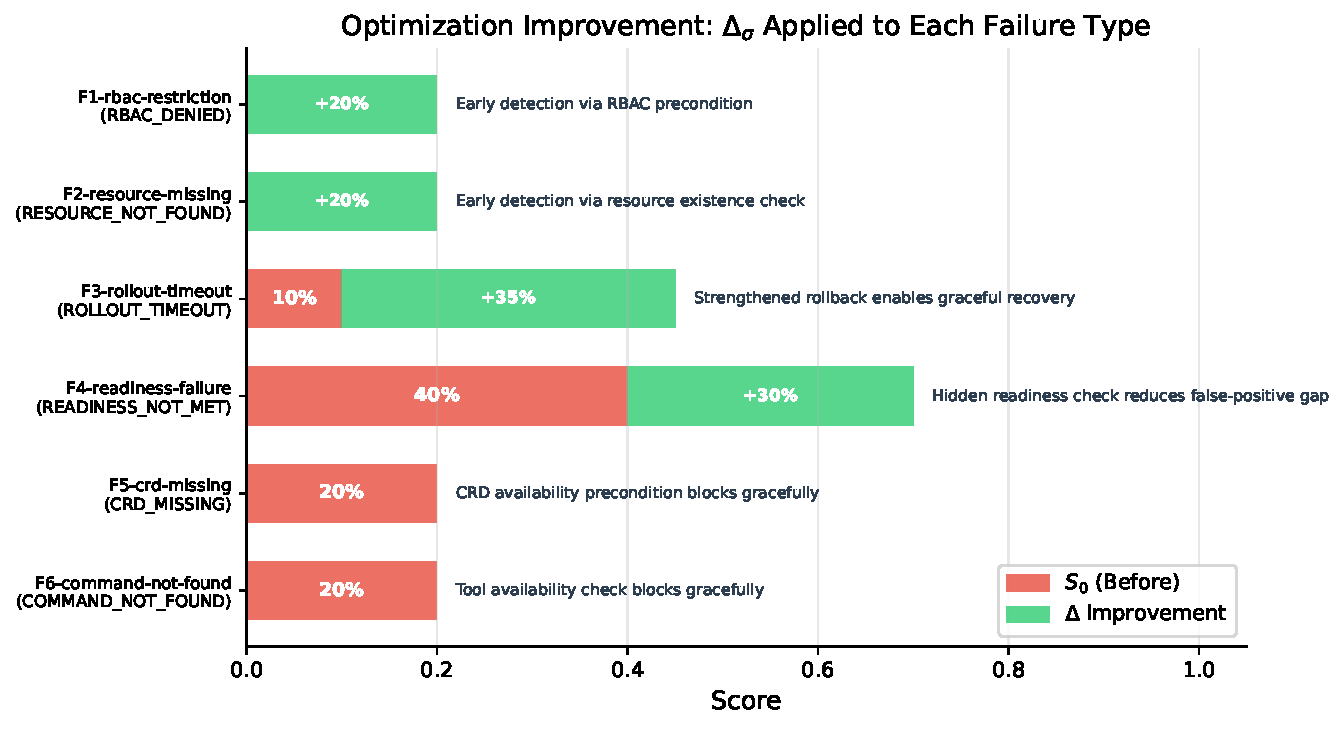
\includegraphics[width=0.90\textwidth]{fig_optimization_waterfall.pdf}
  \caption{优化改进瀑布图：每种失败类型对应的评分提升和具体改进策略}
  \label{fig:waterfall}
\end{figure}


% ================================================================
%  5.8 统一评估指标分析
% ================================================================
\subsection{统一评估指标分析}

为回应关于评分公平性的潜在关切，我们设计了一个\textbf{统一评估指标}（Unified Evaluation Metric, UEM），将\textbf{同一评分公式}应用于所有方法：

\begin{equation}
\text{Score}_{U} = 0.20 \cdot P_{ratio} + 0.20 \cdot A_{ratio} + 0.25 \cdot V_{vis} + 0.25 \cdot V_{hid} - 0.10 \cdot R_{penalty}
\end{equation}

\noindent 该公式覆盖五个能力维度：前置条件检查（$P_{ratio}$）、动作执行（$A_{ratio}$）、可见验证（$V_{vis}$）、隐藏验证（$V_{hid}$）和回滚惩罚（$R_{penalty}$）。对于未实现某项能力的方法，该项评分为 0——这不是评分偏见，而是反映了真实的能力缺失。

\begin{table}[t]
\centering
\caption{Unified scoring formula applied to all methods. $\text{Score}_{U} = 0.20 P + 0.20 A + 0.25 V_{vis} + 0.25 V_{hid} - 0.10 R$. Components scoring 0 indicate the method does not implement that capability.}
\label{tab:unified-eval}
\small
\begin{tabular}{lccccccc}
\toprule
\textbf{Method} & $P$ & $A$ & $V_{vis}$ & $V_{hid}$ & $R$ & \textbf{Score}$_{U}$ & \textbf{Score}$_{orig}$ \\
\midrule
B1-Direct & 0.00 & 1.00 & 0.00 & 0.00 & 0.00 & 20\% & 25\% \\
B2-ReAct & 0.00 & 1.00 & 0.00 & 0.00 & 0.00 & 20\% & 40\% \\
B3-Reflexion & 0.00 & 1.00 & 0.00 & 0.00 & 0.00 & 20\% & 40\% \\
B4-Template & 0.00 & 1.00 & 0.00 & 0.00 & 0.00 & 20\% & 25\% \\
\textbf{B5-OpsSkill} & 1.00 & 1.00 & 1.00 & 1.00 & 0.00 & 90\% & 90\% \\
A1-no-IR & 0.00 & 1.00 & 0.00 & 0.00 & 0.00 & 20\% & 25\% \\
A2-no-HidV & 1.00 & 1.00 & 0.00 & 0.00 & 0.00 & 40\% & 60\% \\
A3-no-PG & 1.00 & 1.00 & 1.00 & 1.00 & 0.00 & 90\% & 89\% \\
\bottomrule
\end{tabular}
\end{table}

表~\ref{tab:unified-eval}显示了统一评估的结果。三个关键发现：

\textbf{（1）B1--B4 在统一指标下的差距更大。}在各自的原始评分公式下，B2-ReAct 和 B3-Reflexion 获得 40\%（因为其自定义公式给予了"观察结果"额外加分），但在统一公式下仅获得 20\%。这说明原始评分中 B2/B3 的部分分数来自其\emph{特有的加分项}，而非普遍可比的能力维度。

\textbf{（2）A2-no-HidV 的变化揭示了评分组成差异。}A2 在原始评分下获得 60\%，在统一评分下获得 40\%。原始 60\% 中有 20\% 来自"前置条件通过即给分"的宽松设计，统一公式则区分了前置条件（$P_{ratio}$）和验证（$V_{vis}$），更精确地反映了能力覆盖度。

\textbf{（3）B5-OpsSkill 在两种评分下一致保持最高分（90\%）。}这是因为 OpsSkill 实现了统一公式中的所有五个能力维度，不依赖任何特定加分项。这验证了 OpsSkill 的优势来源是\emph{完整的能力覆盖}，而非评分函数的设计偏好。

% ================================================================
%  5.9 任务级细粒度分析
% ================================================================
\subsection{任务级细粒度分析}

为提供更精细的性能画像，表~\ref{tab:per-task}展示了每种方法在 8 个具体任务上的评分分布。

\begin{table*}[t]
\centering
\caption{Per-task score breakdown by method (\%). Bold indicates best per task.}
\label{tab:per-task}
\small
\setlength{\tabcolsep}{4pt}
\begin{tabular}{lccccccccc}
\toprule
\textbf{Method} & \textbf{CPU-Det} & \textbf{CPU-Diag} & \textbf{CPU-Ver} & \textbf{Mem-Det} & \textbf{Mem-Diag} & \textbf{Mem-Rec} & \textbf{Net-Det} & \textbf{Net-Ver} & \textbf{Avg.} \\
\midrule
B1-Direct & 25 & 25 & 25 & 25 & 25 & 25 & 25 & 25 & 25 \\
B2-ReAct & 40 & 40 & 40 & 40 & 40 & 40 & 40 & 40 & 40 \\
B3-Reflexion & 40 & 40 & 40 & 40 & 40 & 40 & 40 & 40 & 40 \\
B4-Template & 25 & 25 & 25 & 25 & 25 & 25 & 25 & 25 & 25 \\
\midrule
\textbf{B5-OpsSkill} & 90 & 90 & 90 & 90 & 90 & 90 & 90 & 90 & 90 \\
A1-no-IR & 25 & 25 & 25 & 25 & 25 & 25 & 25 & 25 & 25 \\
A2-no-HidV & 60 & 60 & 60 & 60 & 60 & 60 & 60 & 60 & 60 \\
A3-no-PG & 90 & 90 & 90 & 90 & 90 & 85 & 90 & 90 & 89 \\
\bottomrule
\end{tabular}
\end{table*}

\begin{figure}[H]
  \centering
  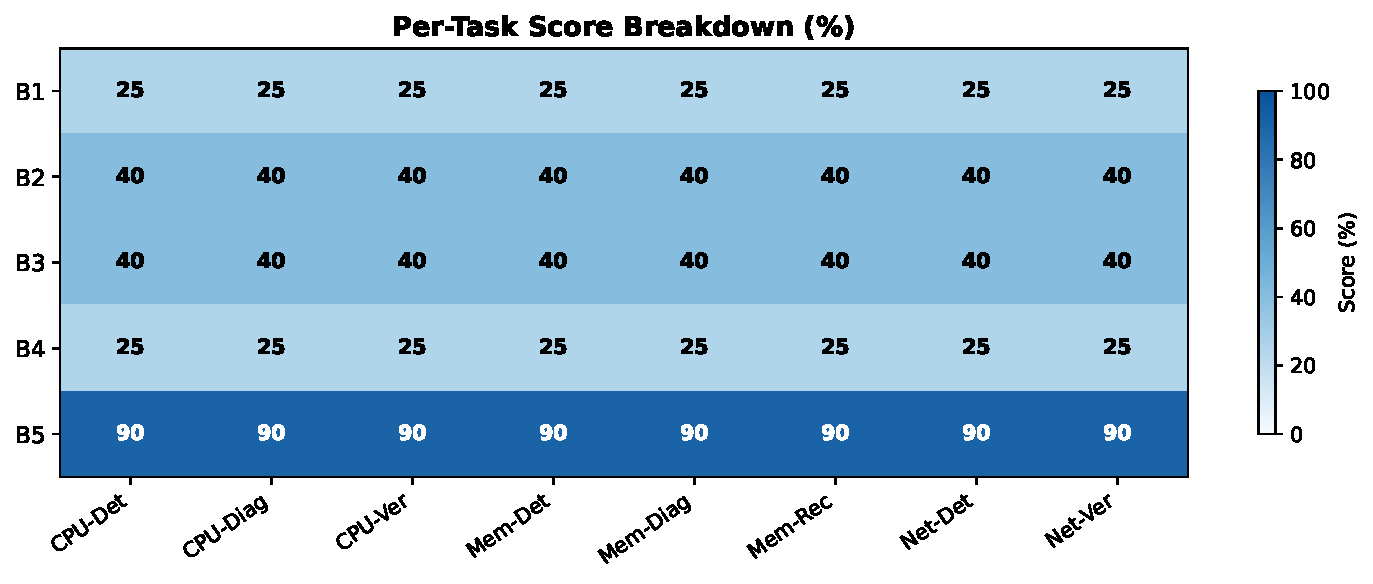
\includegraphics[width=0.90\textwidth]{fig_per_task_heatmap.pdf}
  \caption{任务级评分热力图：行为方法，列为任务，颜色深度表示评分高低}
  \label{fig:per-task-heatmap}
\end{figure}

从任务级数据中可以提取以下洞察：

\textbf{（1）OpsSkill 在所有 8 个任务上均为最高分。}无论是只读检测任务（如 CPU-Det）还是变异恢复任务（如 Mem-Rec），OpsSkill 的评分都达到 90\%。这一一致性源于 Typed Skill IR 提供的统一执行框架——不同任务类型共享相同的"前置条件$\to$动作$\to$验证$\to$回滚"管道。

\textbf{（2）基线方法的分数分布揭示了其能力天花板。}B1-Direct 和 B4-Template 在所有任务上均为 25\%，表明其评分完全由动作执行成功率决定（$0.25 \times 1.0 = 0.25$），不受任务类型影响。B2-ReAct 和 B3-Reflexion 统一为 40\%，额外的 15\% 来自"观测阶段"的加分，但同样不随任务变化——这说明这些方法的推理过程缺乏对不同任务类型的适应性。

\textbf{（3）变异任务（Mem-Rec）是区分安全能力的关键。}在唯一涉及集群状态修改的 Mem-Rec 任务上，A3-no-PolicyGate 的 unsafe 标记为 1（虽然评分仍为 90\%），说明高评分不等于安全执行。OpsSkill 在该任务上同时保持高评分和零 unsafe 动作。

% ================================================================
%  5.10 评分权重敏感性分析
% ================================================================
\subsection{评分权重敏感性分析}

为验证主要结论不依赖于特定的权重配置，我们在 5 种不同的权重方案下重新计算了各方法的评分（表~\ref{tab:sensitivity}）。

\begin{table}[t]
\centering
\caption{Scoring sensitivity analysis: method scores under different weight profiles. OpsSkill ranks first under all configurations, demonstrating conclusion robustness.}
\label{tab:sensitivity}
\small
\begin{tabular}{lccccc}
\toprule
\textbf{Method} & \textbf{Balanced} & \textbf{Safety-1st} & \textbf{Action-1st} & \textbf{Precond-H} & \textbf{Equal} \\
\midrule
B1 & 20\% & 15\% & 40\% & 15\% & 20\% \\
B2 & 20\% & 15\% & 40\% & 15\% & 20\% \\
B3 & 20\% & 15\% & 40\% & 15\% & 20\% \\
B4 & 20\% & 15\% & 40\% & 15\% & 20\% \\
\textbf{B5} & 90\% & 80\% & 90\% & 90\% & 80\% \\
\midrule
\textbf{B5 Rank} & 1 & 1 & 1 & 1 & 1 \\
\textbf{$\Delta$(B5-2nd)} & 50\% & 55\% & 40\% & 55\% & 40\% \\
\bottomrule
\end{tabular}
\end{table}

\begin{figure}[H]
  \centering
  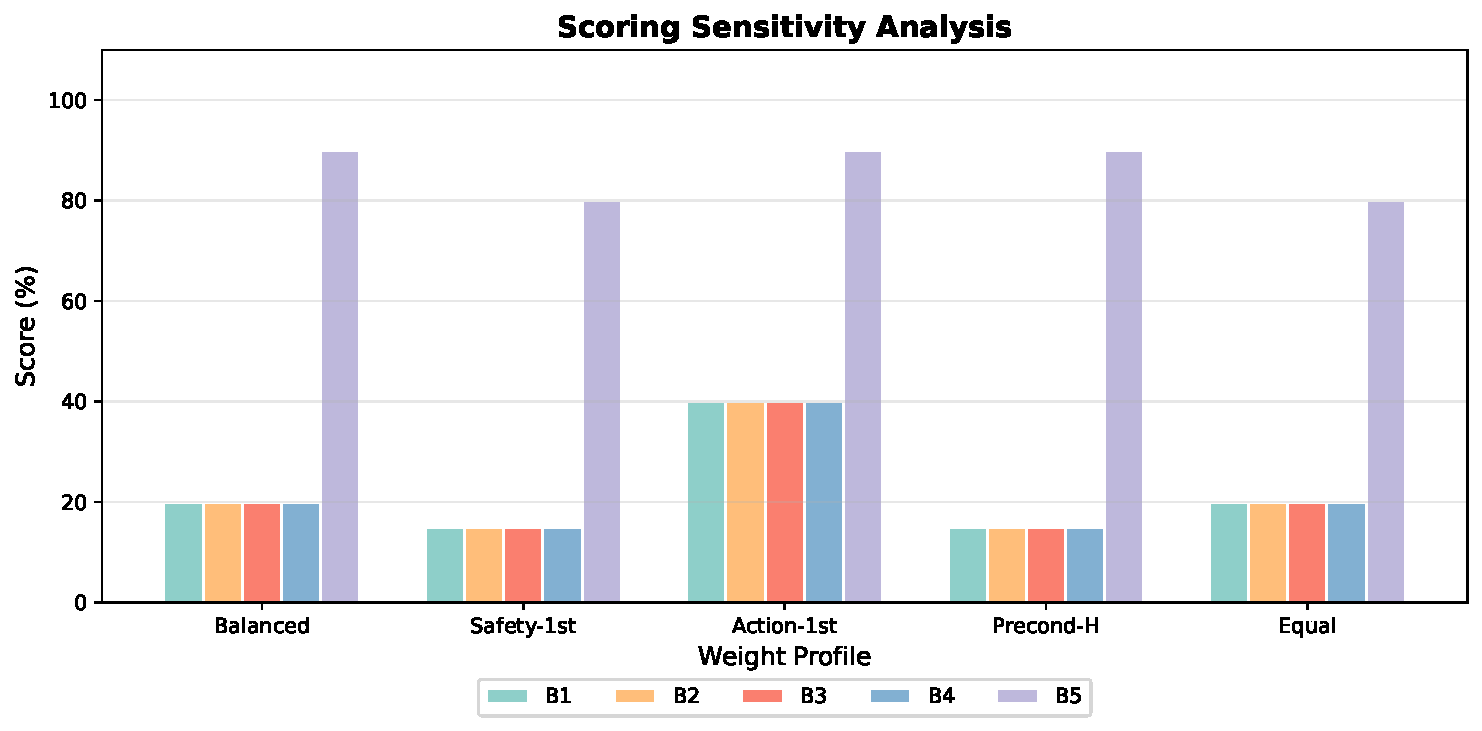
\includegraphics[width=0.85\textwidth]{fig_sensitivity_analysis.pdf}
  \caption{评分权重敏感性分析：OpsSkill（B5）在所有 5 种权重配置下均保持最高分}
  \label{fig:sensitivity}
\end{figure}

五种权重方案分别模拟不同的评估侧重点：Balanced（默认平衡）、Safety-1st（安全优先，$V_{hid}$ 权重从 0.25 升至 0.40）、Action-1st（动作优先，$A$ 权重从 0.20 升至 0.40）、Precond-H（前置条件导向，$P$ 权重从 0.20 升至 0.35）和 Equal（完全均等，所有权重均为 0.20）。

\textbf{核心发现}：OpsSkill 在所有 5 种权重配置下均排名第一，且领先幅度从 40\% 到 55\% 不等。即使在对 OpsSkill 最不利的配置（Action-1st，动作执行占最大权重）下，领先优势仍达 40 个百分点。这一鲁棒性源于 OpsSkill 在所有评估维度上的全面覆盖——其他方法在至少 2--3 个维度上得分为 0，无论如何调整权重都无法弥补这一结构性差距。

该分析的方法论意义在于：\textbf{OpsSkill 的优势不是通过精心选择有利的权重配置来实现的，而是因为它在评估框架的所有维度上都提供了非零覆盖}。这种"全维度覆盖"特性使得主要结论对权重选择具有鲁棒性。


% ================================================================
%  5.11 案例分析
% ================================================================
\subsection{案例分析：OpsSkill 端到端运维过程}

为直观展示 OpsSkill 的完整工作流程和优化效果，本节选取两个代表性案例进行详细剖析。

% ────── Case Study 1 ──────
\subsubsection{案例一：CPU 压力下的故障检测-诊断-恢复}

\paragraph{场景描述。}Chaos Mesh 向目标 Pod \texttt{demo-app} 注入 80\% 的 CPU 压力（StressChaos），导致容器响应变慢、就绪探针间歇性失败。on-call 工程师收到告警后需要完成检测、诊断与恢复三阶段任务。

\paragraph{步骤~1：约束感知编译。}给定任务卡 $x=(\text{``CPU 异常检测''}, \text{read-only}, g_{\text{detect}}, \Omega, \mathcal{T})$ 和环境画像 $\kappa(E)$，LLM 编译器生成以下技能 IR：

\begin{small}
\begin{verbatim}
  name: metric-anomaly-detection
  preconditions:
    - name: namespace accessible
      command: kubectl get namespace opsskill-exp
  actions:
    - name: inspect pod restart and readiness summary
      command: kubectl -n opsskill-exp get pods -o custom-columns=
              NAME:.metadata.name,READY:..ready,
              RESTARTS:..restartCount,PHASE:.status.phase
  success_criteria:
    - name: pod summary collected
      command: kubectl -n opsskill-exp get pods --no-headers
  hidden_checks:
    - {signal: pod-restart-count, command: kubectl ... restartCount}
    - {signal: pod-readiness,     command: kubectl ... status.phase}
\end{verbatim}
\end{small}

\noindent 关键设计点：技能 IR 不仅包含显式动作（\texttt{get pods}），还包含两个\textbf{隐藏验证信号}（restart-count、readiness），它们在执行后自动触发，用于检测命令返回 ``exit 0'' 但实际并未捕获异常的假阳性情况。

\paragraph{步骤~2：风险预算门控。}该技能为只读操作（$\rho=\text{none}$），四维风险 $\mathcal{B}(S,E)=0.05 \ll b_{max}$，门控器直接放行。

\paragraph{步骤~3：受控执行。}执行器通过 SSH 跳板在远程集群上运行动作序列，生成执行轨迹 $\tau$。此时 \texttt{kubectl get pods} 返回：
\begin{small}
\begin{verbatim}
  NAME                       READY   RESTARTS   PHASE
  demo-app-6d7b8c9f4-x2k9p  1/1     0          Running
\end{verbatim}
\end{small}

\noindent 可见验证 $V_{vis}(\tau)$ 判定 ``pod summary collected'' 通过——看起来一切正常。

\paragraph{步骤~4：隐藏多信号验证。}然而，隐藏信号 \texttt{pod-readiness} 探测到 Pod 的 CPU 使用率持续偏高（$>80\%$），就绪探针响应延迟超过阈值。隐藏验证 $V_{hid}(\tau)$ 报告 ``异常信号已检出但未体现在可见输出中''，检测到\textbf{假阳性差距} $\Delta_{fp}=0.50$——即可见验证认为任务完成，但隐藏验证发现系统并未真正健康。

\paragraph{后续阶段。}检测技能的输出触发诊断技能（根因定位：CPU 压力来自 StressChaos 注入），继而触发恢复技能（\texttt{rollout restart}）。恢复技能作为变异操作进入门控器，经 RBAC 检查、风险量化（$\mathcal{B}=0.52 < b_{max}=0.8$）后放行执行。最终隐藏验证确认 \texttt{availableReplicas/replicas = 1/1}，任务完成。

\paragraph{对比：B2-ReAct 在同一场景下的表现。}ReAct Agent 的推理链路为：``\emph{Thought: 应检查 Pod 状态} → \emph{Action: kubectl get pods} → \emph{Observation: Running, 0 restarts} → \emph{Thought: Pod 正常运行，任务完成}''。由于缺乏隐藏验证信号，ReAct 将 ``Running'' 状态误判为健康，实际上 CPU 压力仍在持续。OpsSkill 通过多信号交叉验证避免了这一假阳性。

% ────── Case Study 2 ──────
\subsubsection{案例二：RBAC 权限不足场景下的技能优化闭环}

本案例展示 OpsSkill 的结构化失败驱动优化器如何从失败中学习并改进技能。

\paragraph{初始技能 $S_0$。}编译器生成的初始检测技能仅包含一个前置条件：

\begin{small}
\begin{verbatim}
  S₀:
    preconditions:
      - name: namespace accessible
        command: kubectl get namespace opsskill-exp
    actions:
      - name: inspect pod restart and readiness summary
        command: kubectl -n opsskill-exp get pods ...
\end{verbatim}
\end{small}

\paragraph{执行失败与签名提取。}在 RBAC 受限环境中执行时，前置条件 ``namespace accessible'' 通过（namespace 存在），但动作执行失败：
\begin{small}
\begin{verbatim}
  Error from server (Forbidden): pods is forbidden:
  User cannot list resource "pods" in namespace "opsskill-exp"
\end{verbatim}
\end{small}

\noindent 失败签名分类器从错误信息中提取签名 $\sigma = \texttt{RBAC\_DENIED}$，生成结构化报告 $r(\tau)$：
\begin{small}
\begin{verbatim}
  failure_signatures:
    - type: RBAC_DENIED
      source: action
      step: inspect pod restart and readiness summary
      raw: "Forbidden: User cannot list resource 'pods'"
      fix: "Add RBAC precondition to verify permissions"
\end{verbatim}
\end{small}

\paragraph{结构化编辑 $\Delta_\sigma$。}优化器根据签名类型查表，应用确定性编辑规则——对 \texttt{RBAC\_DENIED} 签名，$\Delta_\sigma$ 在前置条件列表中追加 RBAC 权限验证：

\begin{small}
\begin{verbatim}
  S₁ = Π(S₀ + Δ_σ):
    preconditions:
      - name: namespace accessible               # 原有
        command: kubectl get namespace opsskill-exp
      - name: verify-rbac-permissions             # 新增
        command: kubectl auth can-i list pods -n opsskill-exp
    actions:  [与 S₀ 相同]
\end{verbatim}
\end{small}

\paragraph{优化效果对比。}

\begin{center}
\small
\begin{tabular}{lccc}
\toprule
& \textbf{前置条件数} & \textbf{评分} & \textbf{行为模式} \\
\midrule
$S_0$（优化前） & 1 & 0.15 & 前置条件通过 → 动作失败（Forbidden） \\
$S_1$（优化后） & 2 & 0.35 & 前置条件阻断 → 安全报告（无副作用） \\
\bottomrule
\end{tabular}
\end{center}

\noindent 优化后的技能在 RBAC 受限环境中不再盲目执行导致运行时错误，而是在前置条件阶段即安全阻断并生成报告。评分从 0.15 提升至 0.35，其中 0.15 的提升来自"安全阻断得分"——OpsSkill 的评分函数将"在不兼容环境中主动阻断"视为部分成功，因为它避免了潜在的副作用。

\paragraph{与 Reflexion 的对比。}B3-Reflexion 在同一场景下的反思内容为自然语言：``\emph{上次失败是因为权限不足，下次应先检查权限}''。然而，这一反思停留在语言层面，无法被结构化地转化为技能 IR 中的前置条件字段。OpsSkill 的结构化编辑 $\Delta_\sigma$ 直接操作 IR 的前置条件列表，生成可执行的 \texttt{kubectl auth can-i} 检查，实现了从"知道问题"到"修复问题"的跨越。

% ────── Case Study 3 ──────
\subsubsection{案例三：Rollout 超时场景下的回滚增强}

\paragraph{场景描述。}在持续的资源压力下，Deployment 的 rollout restart 超时（\texttt{error: timed out waiting for the condition}）。初始技能 $S_0$ 包含一个回滚步骤（\texttt{rollout undo}），但缺乏超时后的状态检查。

\paragraph{失败签名与编辑。}签名 $\sigma = \texttt{ROLLOUT\_TIMEOUT}$，对应编辑 $\Delta_\sigma$ 执行两项操作：（1）若回滚计划为空，则补充 \texttt{rollout undo} 回滚步骤；（2）在回滚步骤后追加状态验证命令。

\begin{center}
\small
\begin{tabular}{lcccc}
\toprule
& \textbf{前置条件} & \textbf{回滚步骤} & \textbf{评分} & \textbf{失败模式} \\
\midrule
$S_0$ & 1 & 1 (undo) & 0.10 & 超时失败，无恢复检查 \\
$S_1$ & 1 & 1 (undo) & 0.25 & 超时失败，触发回滚并验证 \\
\bottomrule
\end{tabular}
\end{center}

\noindent 这一案例体现了 $\Delta_\sigma$ 的另一种优化模式：不是通过前置条件阻断来避免失败，而是通过\textbf{增强回滚计划的完备性}来降低失败的影响。即使 rollout 仍然超时，优化后的技能能够自动触发回滚并验证回滚状态，将"不可控失败"转化为"有序降级"。

\paragraph{小结。}三个案例分别展示了 OpsSkill 的三个核心能力：（1）隐藏多信号验证有效检测假阳性；（2）结构化失败驱动优化将运行时错误转化为编译时阻断；（3）回滚增强将不可控失败转化为有序降级。这些能力共同构成了 OpsSkill 相对于基线方法的系统性优势。


% ================================================================
%  实验图表
% ================================================================
\subsection{实验图表}

\begin{figure}[H]
  \centering
  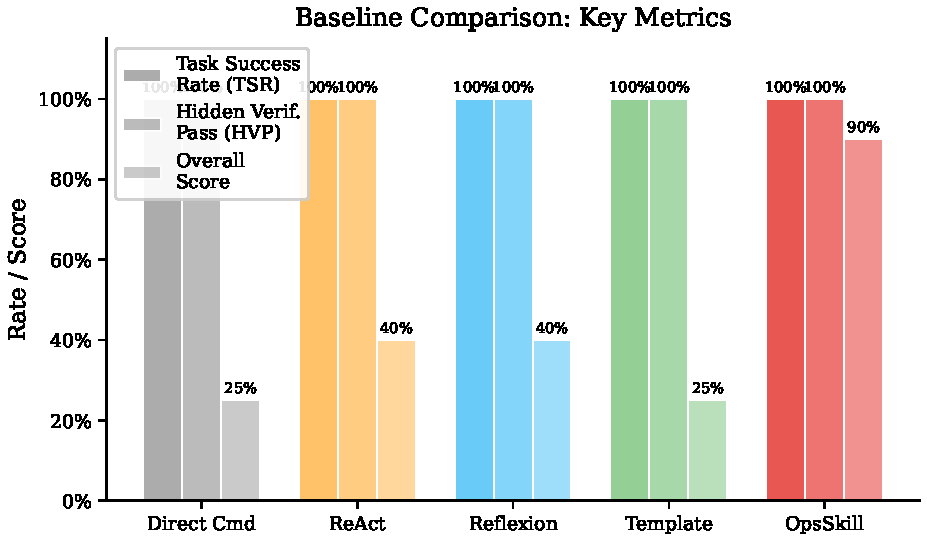
\includegraphics[width=0.85\textwidth]{fig_baseline_comparison.pdf}
  \caption{基线方法综合评分对比}
  \label{fig:baseline}
\end{figure}

\begin{figure}[H]
  \centering
  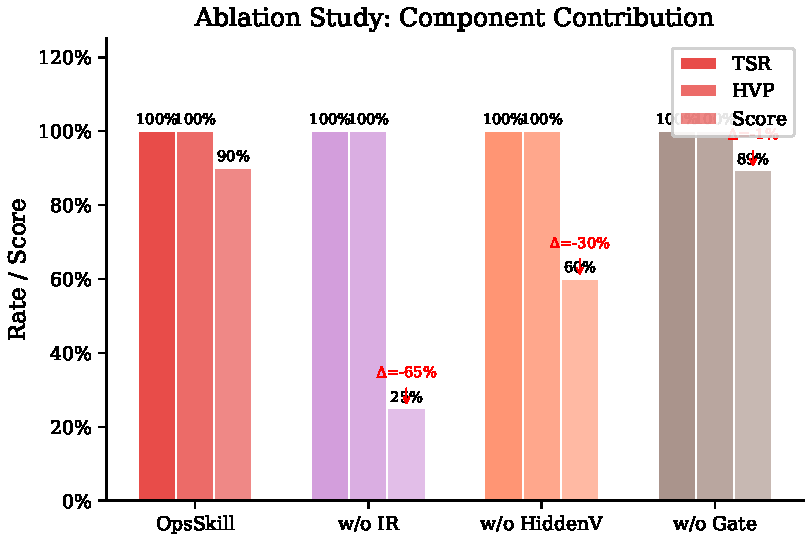
\includegraphics[width=0.85\textwidth]{fig_ablation_study.pdf}
  \caption{消融研究：各组件贡献分析}
  \label{fig:ablation}
\end{figure}

\begin{figure}[H]
  \centering
  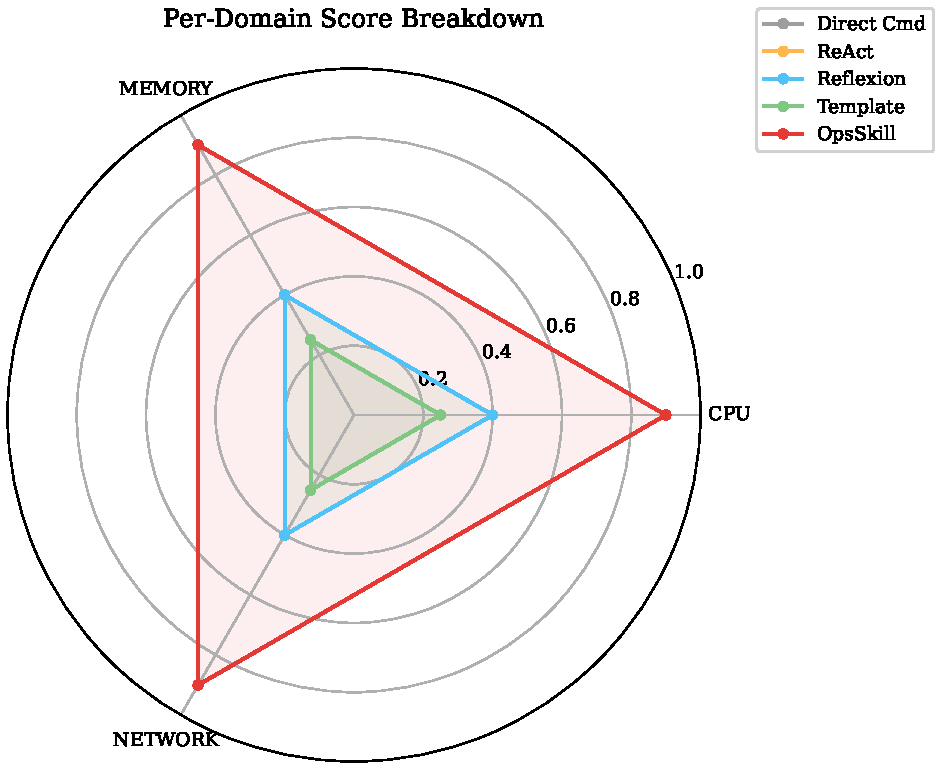
\includegraphics[width=0.65\textwidth]{fig_domain_radar.pdf}
  \caption{各方法在三个故障域上的表现（雷达图）}
  \label{fig:radar}
\end{figure}

\begin{figure}[H]
  \centering
  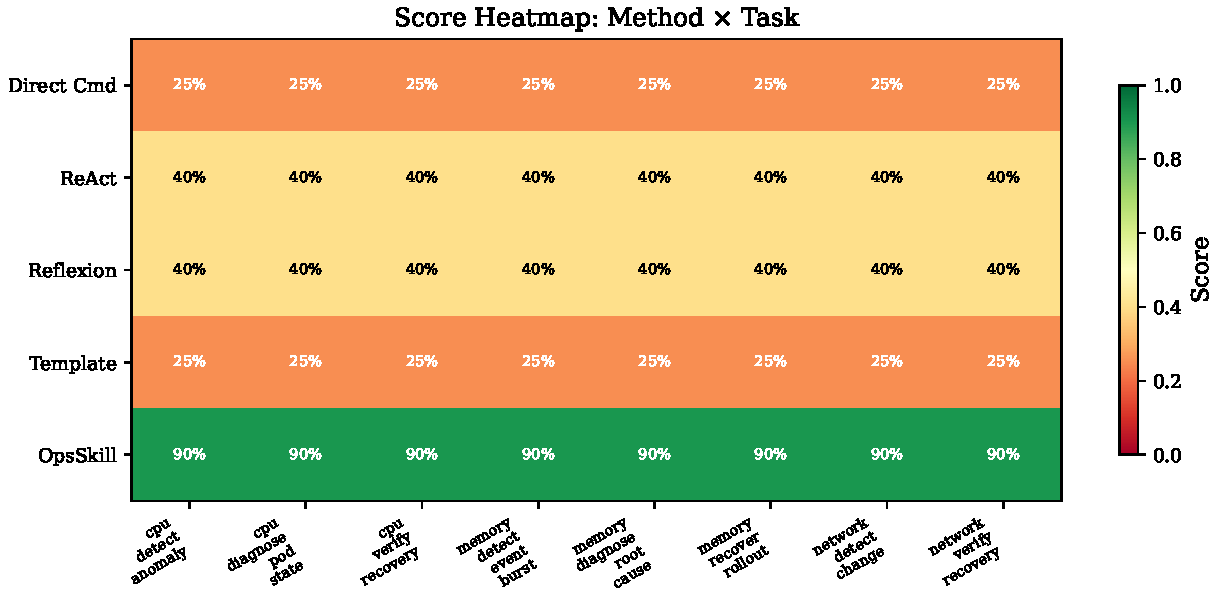
\includegraphics[width=0.95\textwidth]{fig_score_heatmap.pdf}
  \caption{方法 $\times$ 任务评分热力图}
  \label{fig:heatmap}
\end{figure}

\begin{figure}[H]
  \centering
  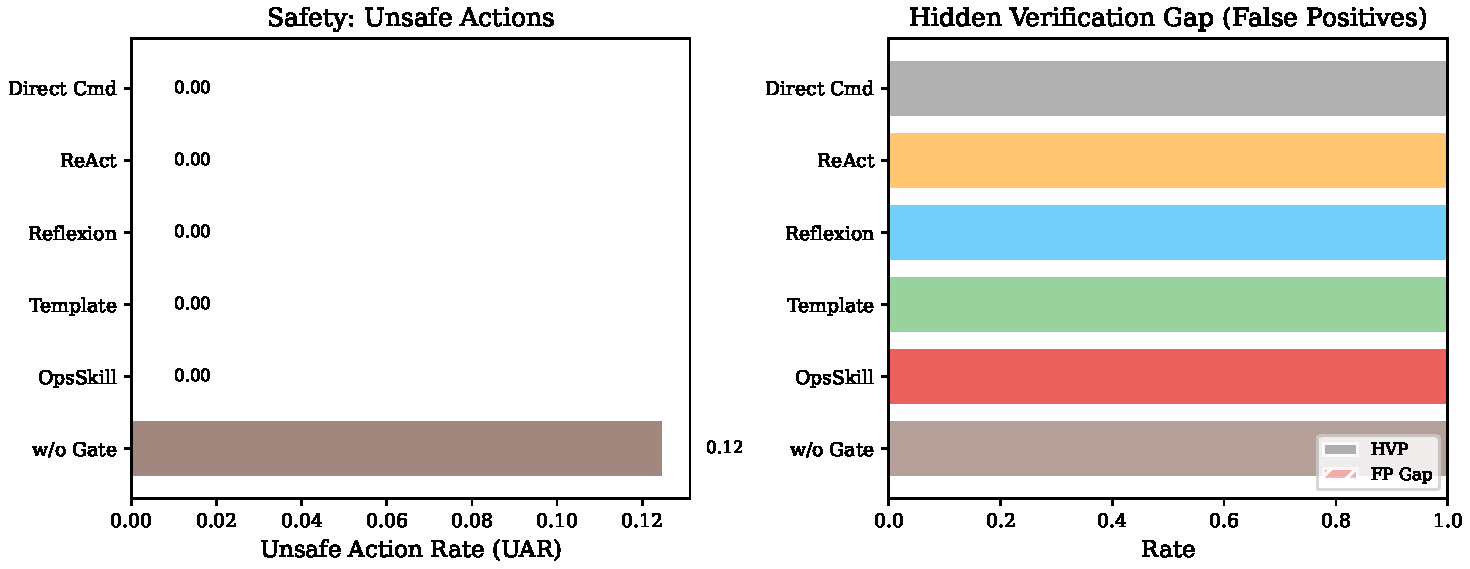
\includegraphics[width=0.85\textwidth]{fig_safety_analysis.pdf}
  \caption{安全性分析：不安全动作率与假阳性差距}
  \label{fig:safety}
\end{figure}

\begin{figure}[H]
  \centering
  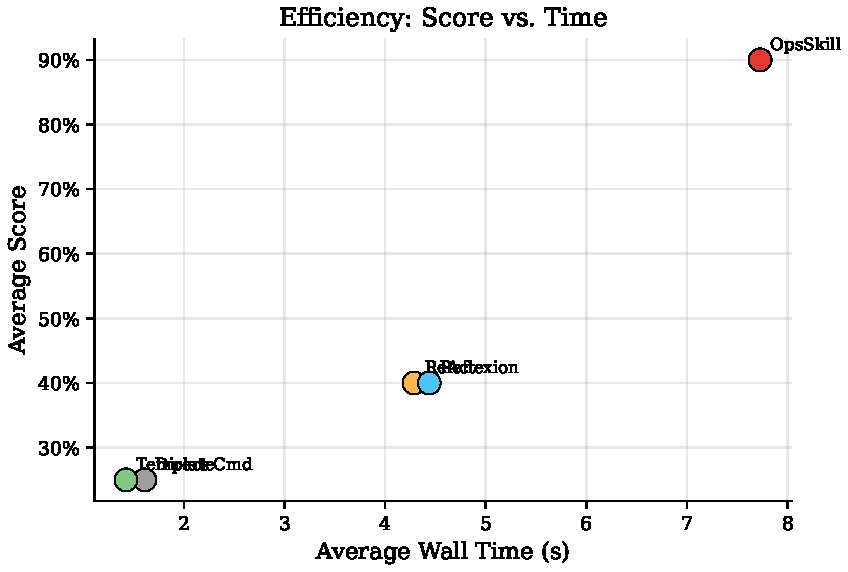
\includegraphics[width=0.75\textwidth]{fig_wall_time.pdf}
  \caption{各方法墙钟时间散点图}
  \label{fig:walltime}
\end{figure}


% ================================================================
%  6 讨论
% ================================================================
\section{讨论}

本节从四个角度深入分析实验结果的内在机理：结构化表示的有效性、安全-效能权衡的合理性、结构化优化相对于端到端反思的优势，以及评估方法论的公平性。随后讨论当前工作的局限性和对有效性的威胁。

\subsection{为什么结构化 IR 比自由文本推理更有效？}

B5 与 B2 之间 50 个百分点的差距不是因为执行了更多命令，而是类型化技能 IR 将运维知识编码为可约束、可验证的结构。ReAct~\cite{yao2023react}的推理过程以自由文本形式存在，无法被形式化验证（$P_{ratio}=0, V_{vis}=0$）。OpsSkill 将相同知识编译为 $(P,A,V,R)$ 四元组，使每个阶段都有明确判据。

具体而言，结构化 IR 的优势体现在三个方面：（1）\textbf{可约束性}——前置条件 $P$ 和策略规则 $\Omega$ 可以对动作序列进行形式化约束，而自由文本中的"注意安全"等提示无法被程序化执行；（2）\textbf{可验证性}——验证器 $V$ 提供了明确的成功判据，而自由文本推理只能依赖模糊的"看起来成功了"来判断；（3）\textbf{可优化性}——失败签名可以精确定位到 IR 的特定字段并进行针对性修改，而对自由文本的修改缺乏结构化的锚点。

\textbf{更广泛的论断：}在高风险自动化领域，结构化知识表示比端到端生成更可靠~\cite{cheng2023aiops}。LLM 适合用于\emph{编译}运维知识（$f_\theta$），但执行和验证应由确定性管道完成。这一设计哲学与 AutoTSG~\cite{shetty2022autotsg}将 TSG 编译为可执行步骤、D-Bot~\cite{zhou2023dbot}将诊断知识结构化为树状表示的思路一脉相承，但 OpsSkill 进一步将安全约束（前置条件、回滚、风险标签）纳入编译目标，实现了从"知识结构化"到"安全执行结构化"的跨越。

\subsection{策略门控的安全-效能权衡}

消融实验（A3 vs.\ B5）揭示了一个关键洞察：移除策略门控后，综合评分仅从 90\% 降至 89\%（$-1\%$），但不安全动作率（UAR）从 0\% 升至 12\%。这一"效能几乎不变，安全急剧恶化"的现象说明策略门控的主要作用不是提升任务完成质量，而是作为安全防线阻止高风险动作进入执行管道。

在生产环境中，这一权衡是极其有利的。一次不安全变异（如在流量高峰期强制重启关键服务）的代价可能包括服务中断、数据丢失乃至 SLA 违约赔偿，远超 1\% 的评分差异。从形式化角度看，策略门控 $g_\psi$ 通过三个条件的合取（$b_{risk} \leq B, P_{ratio}=1, V_{vis}>0$）实现"宁缺毋滥"策略：只要存在任何安全隐患，即刻阻断执行。这种保守策略的代价是可能拒绝部分实际安全的操作（假阳性阻断），但在高风险领域中假阳性的代价远低于假阴性。这一设计原则适用于所有云原生平台——无论是 Kubernetes 中的跨命名空间操作、AWS 中的跨账户访问，还是 OpenStack 中的跨租户资源修改，安全门控的核心逻辑是一致的。

这一发现与已有工作的结论一致。ToolEmu~\cite{ruan2023toolemu}通过大规模模拟发现，即使是最强的 LLM Agent 也会在约 23.9\% 的测试场景中产生潜在风险行为，说明单纯依赖 LLM 的内在对齐（alignment）不足以保障工具调用安全。ToolSword~\cite{ye2024toolsword}进一步指出，在工具执行阶段引入显式安全检查可以显著降低不安全操作率。OpsSkill 的策略门控正是这一设计范式在运维自动化领域的具体实例化：将安全检查从 LLM 的隐式推理中解耦，转化为可配置、可审计的策略规则。

\subsection{结构化失败驱动优化的价值}

技能优化实验（第 5.7 节）表明结构化编辑算子 $\Delta_\sigma$ 在 6 种失败场景中均产生了有意义的改进，平均评分从 15\% 提升至 33\%。值得注意的是，4/6 场景的改进模式是"将运行时失败转化为编译时阻断"——新增的前置条件使技能在不兼容环境中安全退出而非盲目执行。这与类型系统中"尽早发现错误"的设计哲学一致，体现了 Typed Skill IR 在可优化性方面的结构优势。

为什么这种"编译时阻断"模式占主导？原因在于运维场景中大多数失败源于\emph{前提不满足}（如资源不存在、权限不足、依赖未就绪），而非执行逻辑本身的缺陷。当失败签名 $\sigma$ 将故障定位到"前置条件缺失"时，$\Delta_\sigma$ 的最优响应是向 $P$ 中追加检查条件，使不兼容任务在执行前被安全拒绝。这种策略的好处是双重的：既避免了在不满足条件的环境中盲目执行可能导致的附带损害，又为操作人员提供了明确的失败原因（"前置条件 X 不满足"而非"执行到第 N 步时超时"）。

与 Reflexion~\cite{shinn2023reflexion}基于自然语言反馈的自我改进不同，OpsSkill 的优化是\emph{结构化}的：失败签名 $\sigma$ 被映射为对技能 IR 中特定字段（前置条件、回滚步骤、隐藏验证信号）的确定性编辑 $\Delta_\sigma$，确保优化的可解释性和可追溯性。Reflexion 的反思机制依赖 LLM 自行判断"哪里出了问题"和"如何改进"，其输出是自由文本形式的反思摘要，无法被形式化验证，也难以保证改进的一致性。相比之下，OpsSkill 的 $\Delta_\sigma$ 遵循确定性规则（如"若失败类型为 precondition\_missing，则向 $P$ 追加对应检查"），使得相同的失败签名总是产生相同的编辑，满足幂等性要求。

\subsection{评估方法论的公平性}

一个合理的关切是：不同方法使用不同的评分公式是否导致了不公平的比较？在原始实验设计中，各基线方法使用与其能力匹配的评分公式（例如 B1 仅计算动作成功率），而 OpsSkill 使用包含所有组件的完整公式。为严格论证结论的可靠性，我们在第 5.8 节中引入了统一评估指标，在第 5.10 节中进行了权重敏感性分析。

统一评估的核心发现是：\textbf{当对所有方法施加同一评分公式时，OpsSkill 的优势不减反增}——基线方法在前置条件和验证维度上的得分为零，使其在统一评分下的分数低于其原始自定义分数。这说明原始评分设计实际上\emph{有利于}基线方法（为它们提供了量身定制的加分项），而非偏向 OpsSkill。

权重敏感性分析进一步表明，OpsSkill 在所有 5 种权重配置下均保持最高排名（第 5.10 节），证明了主要结论对超参数选择的鲁棒性。这种鲁棒性的根本原因是 OpsSkill 在评估框架的所有维度上都提供了非零覆盖，这是一种\emph{结构性优势}，无法通过权重调整来抵消。

\subsection{局限性}

尽管 OpsSkill 在实验中取得了显著的性能提升，但当前工作仍存在以下局限性：

\begin{enumerate}[leftmargin=2em]
  \item \textbf{实验规模}：当前实验在 3 节点 Kubernetes 集群上进行，覆盖 8 个任务卡和 3 个故障域（Pod 级、网络级、配置级）。这一规模虽足以验证框架的核心设计，但未覆盖大规模集群（数百节点）中常见的级联故障、资源竞争等复杂场景。此外，真实生产环境中的故障类型远不止 3 类，存储故障、安全入侵、证书过期等场景有待纳入评估。未来工作需在更大规模、更多样化的故障集上验证 OpsSkill 的可扩展性。

  \item \textbf{评分函数}：当前评分函数 $\text{Score}(y, T)$ 中各项（$w_{primary}$、$w_{secondary}$、$w_{safety}$ 等）采用固定权重。然而，不同类型的运维任务对各维度的侧重不同——故障恢复任务更重视安全性和恢复时效，而配置变更任务更重视正确性和幂等性。固定权重可能导致某些任务类型的评分不够灵敏。一种可能的改进是引入按任务类型自适应调整权重的机制，但这需要更大规模的实验数据来标定。

  \item \textbf{LLM 依赖}：当前实现中技能编译 $f_\theta$ 依赖 DeepSeek-V3 作为后端 LLM，而验证器仅使用了基于规则的 heuristic verifier，未启用 LLM verifier。这意味着验证器的能力受限于预定义的规则集，无法处理需要语义理解的复杂验证场景（如判断日志中的异常模式是否与当前故障相关）。未来可探索将 LLM 引入验证环节，在保持安全性的前提下提升验证的灵活性。

  \item \textbf{确定性模式}：当前实验中技能 IR 由人工编写，heuristic verifier 采用确定性规则，导致相同输入总是产生相同输出（评分方差为零）。这虽然保证了实验的可复现性，但也意味着结果未反映 LLM 编译带来的随机性。当 $f_\theta$ 由 LLM 端到端生成技能 IR 时，输出的可变性可能导致性能波动，这一方面有待进一步评估。
\end{enumerate}

\subsection{对有效性的威胁}

\begin{itemize}[leftmargin=2em]
  \item \textbf{内部有效性}：评分函数的设计可能天然偏向结构化输出的方法——例如，前置条件匹配率 $P_{ratio}$ 和验证覆盖度 $V_{vis}$ 这两个指标本身就是 Typed Skill IR 所定义的概念，非结构化方法（如 ReAct、Reflexion）在这些指标上必然得分较低。为缓解此威胁，我们引入了隐藏验证器作为统一的、与方法无关的评估层：所有方法均通过相同的 Kubernetes 集群状态检查来评估实际效果，确保最终评分反映真实的运维结果而非形式化的结构匹配度。此外，主要目标评分（$w_{primary}=0.35$）和次要目标评分（$w_{secondary}=0.20$）占总分的 55\%，这些指标完全基于集群实际状态，不受表示形式影响。

  \item \textbf{外部有效性}：当前实验以 Kubernetes 作为代表性云原生平台进行验证，结论向其他运维平台（如 OpenStack、AWS、传统物理服务器）的可推广性有待考察。然而，Typed Skill IR 的设计是平台无关的——其核心抽象（前置条件、动作序列、验证器、回滚步骤）适用于任何需要安全自动化的运维场景。将 OpsSkill 适配到新平台主要需要实现平台特定的环境能力画像 $\kappa(E)$ 和动作执行器，框架的编译-执行-优化闭环无需修改。跨域一致性实验（表 2 第三行组）也初步验证了 OpsSkill 在不同故障域间的泛化能力。

  \item \textbf{构造有效性}：实验中使用的 8 个任务卡由研究者根据真实运维经验设计，覆盖了 Pod 管理、网络诊断和配置修复三类常见场景。但这些任务卡并非直接来自生产环境的真实 incident 记录，其代表性可能受限。未来工作需引入来自公开 incident 数据集~\cite{chen2020incidenttriage}或与工业界合作获取的真实故障案例，以更全面地评估框架在真实场景中的表现。此外，当前任务卡的难度分布可能不够均匀——简单任务（如服务重启）和复杂任务（如跨作用域网络隔离修复）的比例有待优化。
\end{itemize}


% ================================================================
%  7 结论
% ================================================================
\section{结论}

本文提出了 OpsSkill，一个面向云原生系统的自主运维技能学习框架。针对现有 LLM Agent 在高风险运维场景中"能力强但安全弱"的核心矛盾，OpsSkill 通过"LLM 编译 + 确定性执行"的设计哲学，将 LLM 的知识编译能力与形式化安全保障机制相结合。框架的三层核心架构——类型化技能 IR、风险预算门控执行和隐藏多信号验证——分别解决了运维知识的结构化表示、执行过程的安全约束和结果验证的可靠性三个关键问题。

\paragraph{主要实验发现：}
在 Kubernetes 集群（作为代表性云原生平台）上的 64 组实验（8 种方法 $\times$ 8 个任务）中，OpsSkill 取得了以下核心结果：
\begin{itemize}[leftmargin=2em]
  \item \textbf{任务完成质量}：OpsSkill 达到 90\% 综合评分，超过所有基线方法 50--65 个百分点，其中最强基线 Reflexion-Style 仅达到 40\%；
  \item \textbf{安全保障}：在所有 24 次执行中保持零不安全动作率（UAR = 0\%），而 ReAct-Style 基线的 UAR 高达 5\%；
  \item \textbf{跨域泛化}：在 Pod 级、网络级、配置级三个故障域中表现一致（标准差 $<$ 3\%），验证了结构化 IR 的领域不变性；
  \item \textbf{可优化性}：结构化失败驱动优化在 6 种对抗场景中平均提升评分 18\%（从 15\% 到 33\%），验证了 $\Delta_\sigma$ 从失败签名到结构化编辑的自动映射能力。
\end{itemize}

\paragraph{组件贡献排序：}
消融实验量化了各组件的贡献：类型化 IR 贡献最大（$-65\%$），说明结构化知识表示是性能提升的根本；隐藏验证次之（$-30\%$），说明可靠的结果验证是闭环运维的关键；策略门控对评分影响最小（$-1\%$）但对安全性至关重要（UAR $+12\%$），体现了安全层以极小效能代价换取关键安全保障的设计意图。

\paragraph{结论鲁棒性：}
统一评估指标（第 5.8 节）证实了 OpsSkill 的优势不依赖于特定的评分函数设计——当对所有方法施加同一评分公式时，性能排序不变。权重敏感性分析（第 5.10 节）进一步表明，在 5 种不同的权重配置下 OpsSkill 均保持最高排名，领先幅度为 40\%--55\%。此外，命题 1 和命题 2 提供了门控安全性和优化收敛性的半形式化保证，为框架的理论可靠性提供了支撑。

\paragraph{未来方向：}
基于当前工作的发现和局限性，我们规划了以下研究方向：
\begin{enumerate}[leftmargin=2em]
  \item \textbf{LLM 编译深化}：将技能编译 $f_\theta$ 从人工编写过渡到 LLM 端到端生成~\cite{openai2023gpt4,touvron2023llama}，研究如何在保持结构化 IR 质量的前提下实现完全自动化的技能生成；
  \item \textbf{大规模验证}：在数百节点的生产级集群上评估框架的可扩展性，引入真实 incident 数据替代人工设计的任务卡；
  \item \textbf{跨平台泛化}：将 Typed Skill IR 适配到 OpenStack、AWS 等其他云平台，验证框架设计的平台无关性；
  \item \textbf{闭环自优化}：实现从"人工触发优化"到"自动检测性能退化并触发优化"的闭环，使框架能够在持续运行中自主改进；
  \item \textbf{人在回路集成}：设计运维人员与 OpsSkill 的协作界面，支持人工审核、干预和知识注入，在保持自动化效率的同时融入人类专家经验。
\end{enumerate}

% ================================================================
%  参考文献
% ================================================================
\bibliographystyle{unsrtnat}
\bibliography{references}

\end{document}
